% !TEX root = ../gnss_interference_resistant_thesis.tex
\documentclass[main.tex]{subfiles}

\begin{document}

\subsection{GNSS imtuvo matavimai}

GNSS matavimai atlikti naudojant 4 HackRF imtuvus su prijungtomis
4 aktyviomis antenomis išdėstytomis kvadrato formoje $\lambda / 2$
atstumu, kaip pavaizduota \ref{fig:gnss_antenna_patern}~pav.

\begin{figure}[h]
    \begin{centering}
    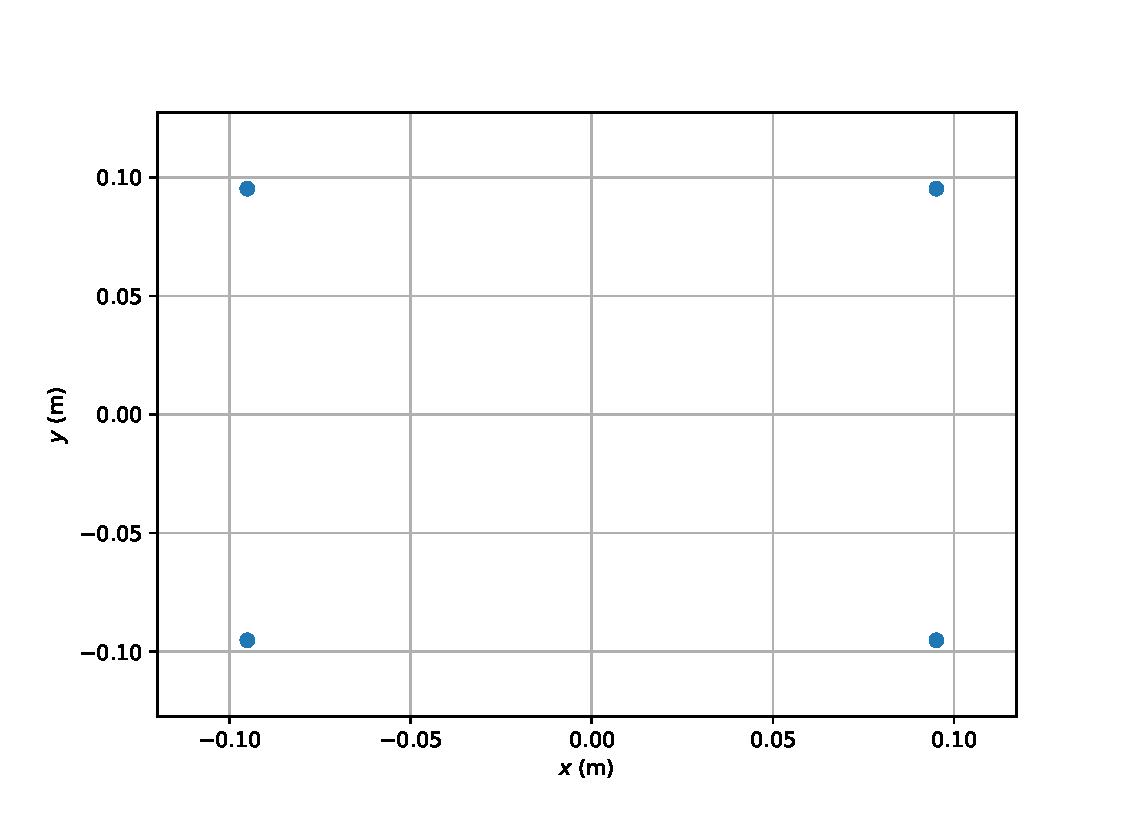
\includegraphics[scale=0.65]{drawings/antenna_pattern}
    \par\end{centering}
    \protect\caption{\label{fig:gnss_antenna_patern}Antenų masyvo, naudoto GNSS imtuvo tyrimams, išdėstymo schema.}
\end{figure}

Visi matavimai atliekami išsisaugant neapdorotus duomenų failus iš kiekvieno
imtuvo atskirai ir duomenų apdorojimas vykdomas šia tvarka:

\begin{enumerate}
    \item Atliekamas duomenų apdorojimas \ref{sec:gnss_doa_block} skyriuje aprašytu bloku;
    \item Atliekamas fazių kalibravimas pasinaudojant vienu iš matomų palydovų;
    \item Pritaikomas MUSIC algoritmas signalų krypčių nustatymui;
    \item Duomenys apdorojami nenaudojant spindulio formavimo;
    \item Duomenys apdorojami taikant spindulio formavimo algoritmą;
\end{enumerate}

\subsubsection{Fazės kalibravimas naudojant GNSS signalą}

Kaip aprašyta ankstesniuose skyriuose, naudojant HackRF SDR imtuvus, kiekvieno
matavimo pradžioje reikalingas fazinis imtuvų kalibravimas. Tam kad supaprastinti
matavimo metodiką, faziniam kalibravimui naudojamas priimamas GPS signalas.

Tam kad būtų galima atlikti kalibravimą, palydovas, naudojamas kalibravimui,
turi būti gerai matomas, bei jis turi būti dangaus skliauto viršuje.
Kai palydovas yra statmenai antenų masyvui, visos priimamos fazės visuose
imtuvuose turi būti lygios 0. Dėl šios priežasties, matavimus reikia
planuotis iš anksto, tuo laiku kai bent vienas palydovas yra
kuo aukščiau virš horizonto. Vieno iš toliau pateiktų matavimų,
palydovų pozicijos pateiktos \ref{fig:gnss_sat_pos_calibartion}~pav.,
kalibravimui naudotas PRN29 palydovas.

\begin{figure}[ht]
    \begin{centering}
    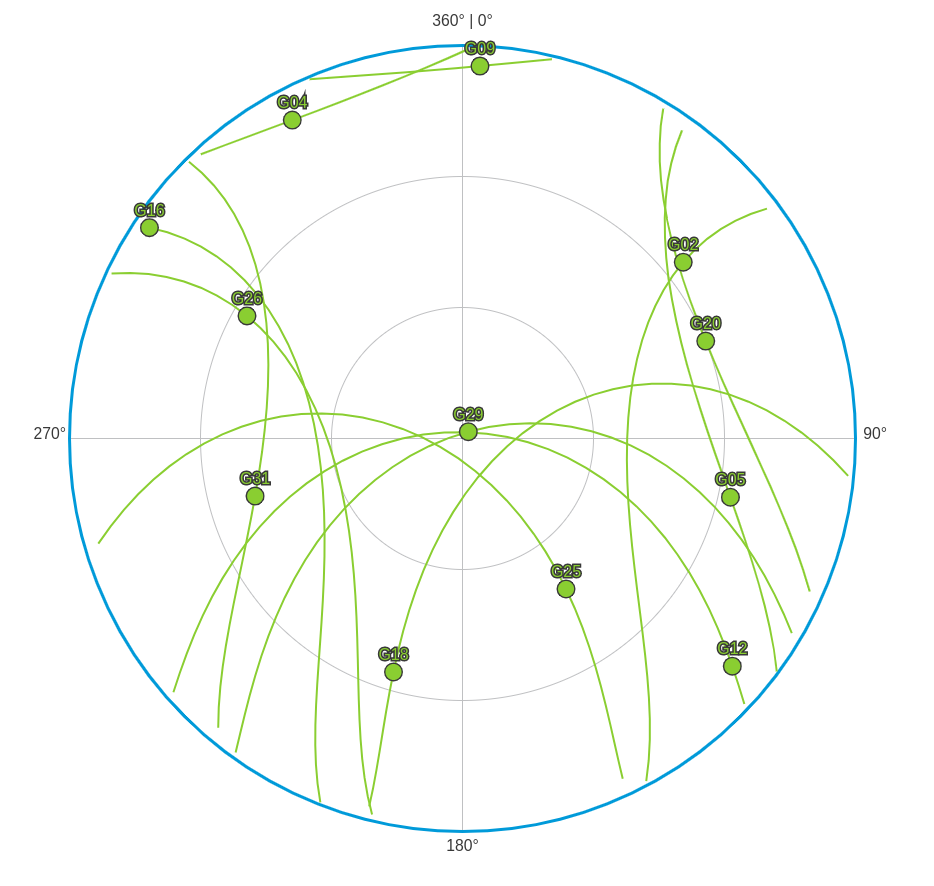
\includegraphics[scale=1.2]{drawings/gnss_sattelites_position}
    \par\end{centering}
    \protect\caption{\label{fig:gnss_sat_pos_calibartion}GPS palydovų pozicijos dangaus skliaute, adresu Saulėtekio al. 9, Vilnius, 2022-05-11 13:20.}
\end{figure}

Kalibravimas atliekamas lyginant vienos iš antenų fazę, su kitų trijų antenų fazėmis.
Atliekamas vidurkio skaičiavimas, gauta vertė atitinka fazės nuokrypį nuo tikrosios
fazės, ši vertė naudojama fazės poslinkiui visuose skaičiavimuose.

Jeigu palydovas nėra statmenas antenų masyvui, pritaikius spindulio formavimo
algoritmą, galime suskaičiuoti fazes kiekvienoje antenoje ir šis pokrypis
yra pridedamas prie nulinės fazės. Fazių kalibravimo pavyzdys pateiktas
\ref{fig:gnss_phase_calibration}~pav.

\begin{figure}[ht]
    \begin{centering}
    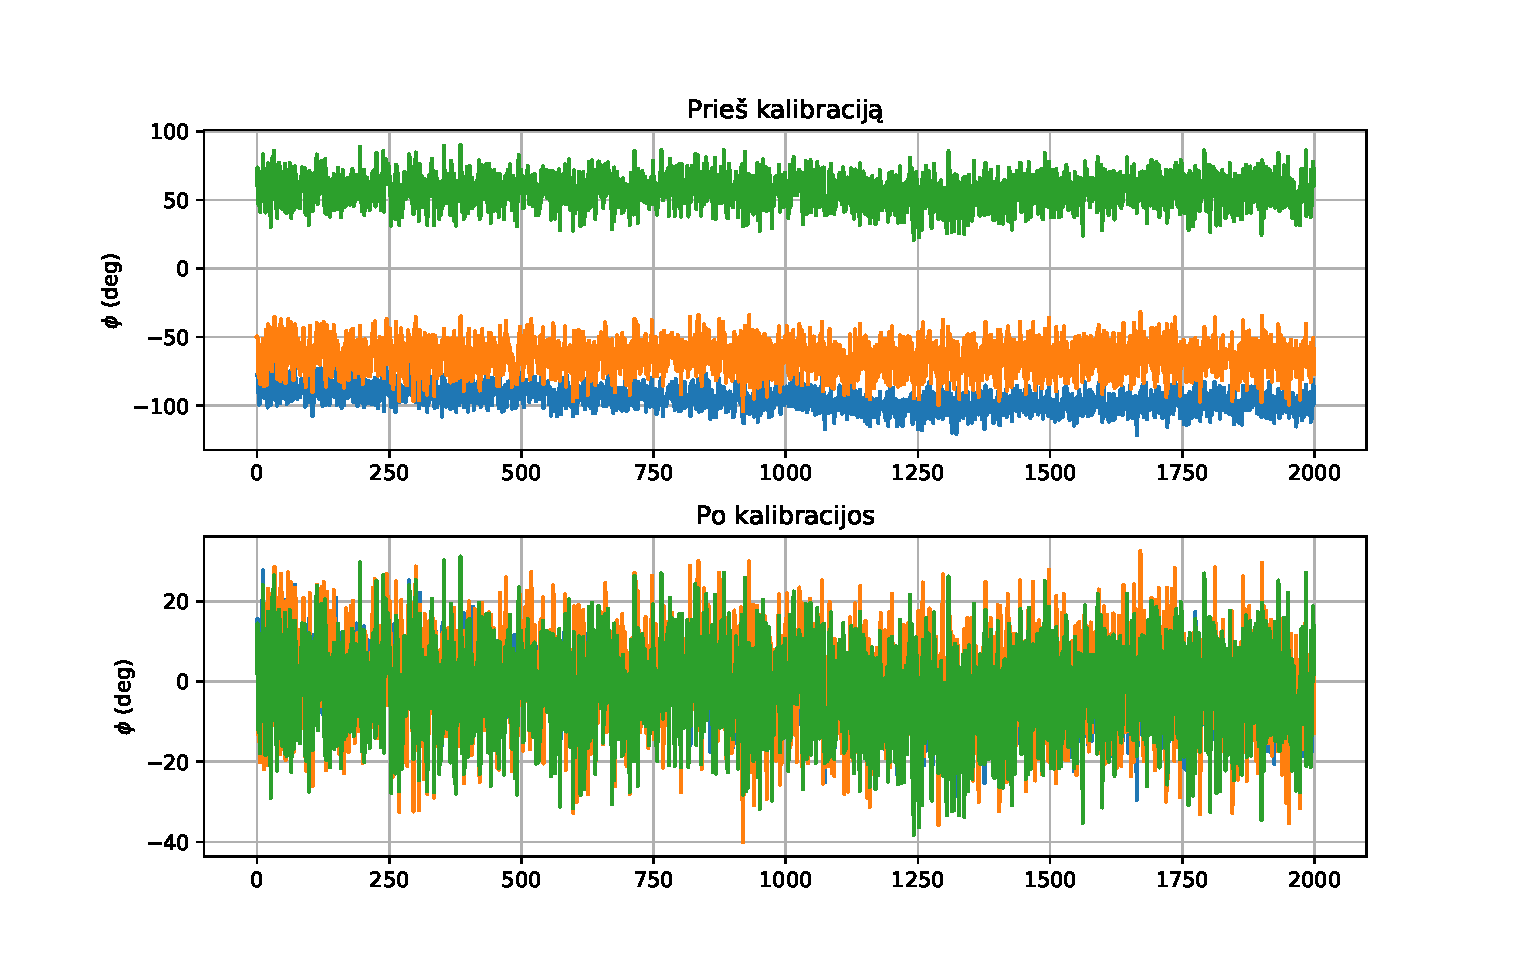
\includegraphics[scale=0.65]{drawings/phase_calibration}
    \par\end{centering}
    \protect\caption{\label{fig:gnss_phase_calibration}PRN29 palydovo priimto signalo fazės kiekviename antenų masyvo elemente, prieš kalibravimą ir po kalibravimo.}
\end{figure}

\subsubsection{GNSS signalų priėmimas kai nėra kliūčių}\label{sec:gnss_meas_no_reflection}

Pirmam matavimui buvo pasirinkta atvira vietovė, kurioje dangaus skliautas nėra blokuojamas
jokių kliūčių. Matavimas buvo atliekamas 10 minučių, fazės kalibravimas atliktas pagal PRN18 palydovą.
\ref{fig:no_reflection_sat_pos}~pav. kairėje pavaizduota matavimų metu buvęs palydovų išsidėstymas
dangaus skliaute. Kadangi PRN18 yra aukščiausiai esantis palydovas, jis buvo pasirinktas
faziniam kalibravimui. Apytikslė matavimų vieta pažymėta raudonu kryžiuku žemėlapyje.
Iš palydovinės nuotraukos galime matyti, kad pasirinktoje vietovėje nėra pastatų,
bei aukštos augalijos.

\begin{figure}[ht]
    \begin{centering}
    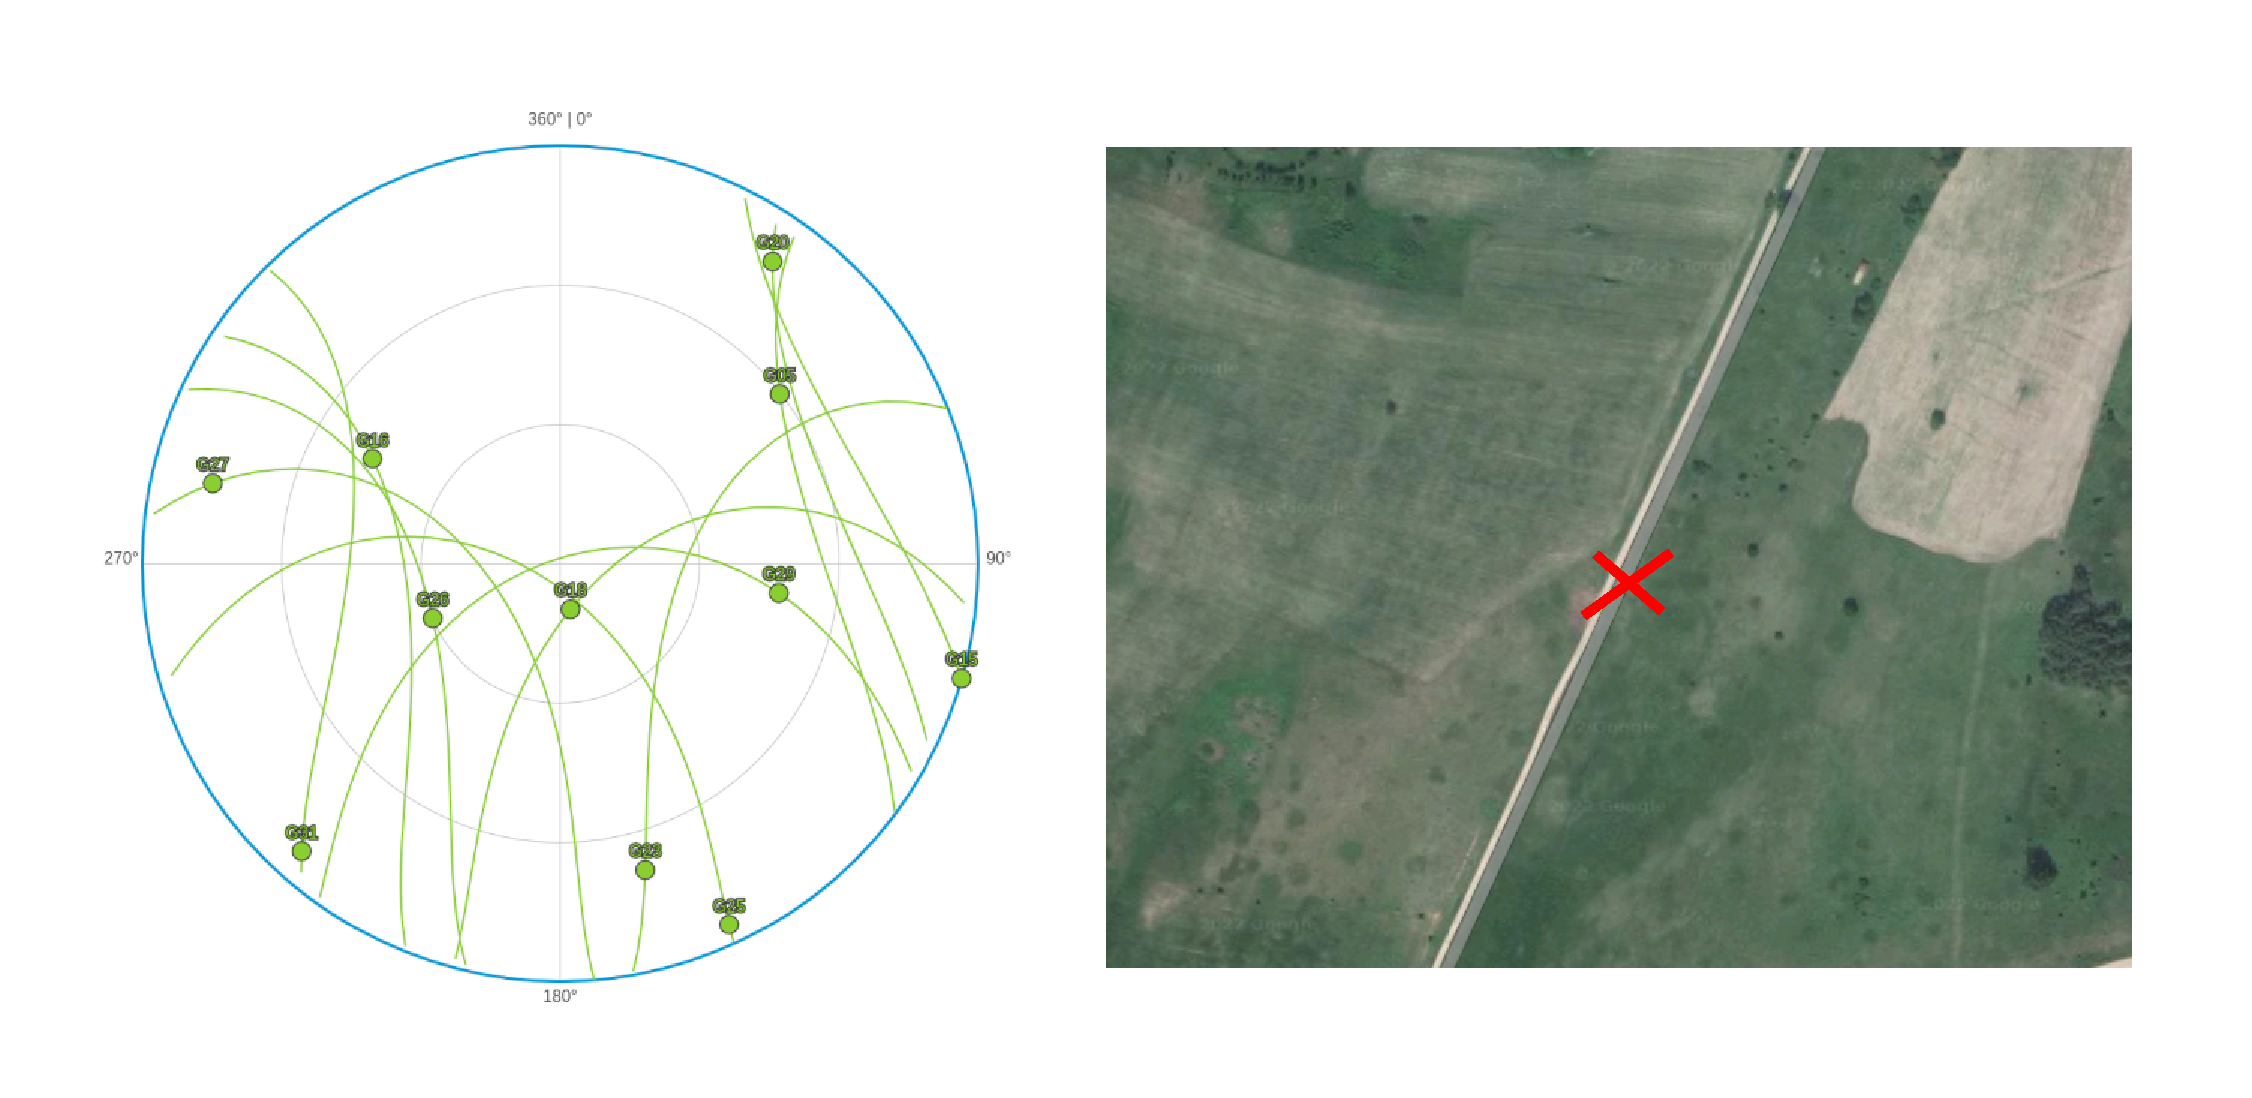
\includegraphics[scale=0.35]{drawings/open_sat_positions.drawio}
    \par\end{centering}
    \protect\caption{\label{fig:no_reflection_sat_pos}Kairėje palydovų išsidėstymas dangaus skliaute matavimų metu, dešinėje matavimo vietovės palydovinė nuotrauka \cite{google_maps}.}
\end{figure}

Pritaikius GNSS signalų apdorojimą aprašytą \ref{sec:gnss_doa_block} skyriuje, gauti
rezultatai pavaizduoti \ref{fig:no_reflection}~pav. Kiekvienas grafikas parodo
individualaus palydovo MUSIC pseudospektro vertę, azimutas rodo nustatytą
pasaulio šalies kryptį, kur 0 atitinka šiaurę, 180/-180 - pietūs. Aukštis rodo palydovo aukštį virš horizonto
laipsniais.
Juodas kryžiukas parodo tikrąja palydovo poziciją, kuri
nustatyta pasinaudojus žinomomis palydovų orbitomis, matavimo data, laiku ir pozicija.

\ref{fig:no_reflection}~pav. visi grafikai turi vieną stiprų maksimumą, kuris atitinka signalo priėmimo kryptį.
Taip pat kadangi yra tik vienas maksimumas, galime daryti išvadą, kad šioje matavimo vietovėje
imtuvas nemato signalo atspindžių ir priima tik tiesioginį palydovo signalą.
PRN18 grafike maksimumas tiksliausiai sutampa su tikrąja palydovo pozicija, kadangi
fazinis kalibravimas buvo atliekama pagal šį palydovą.
Kitų palydovų tikrojo pozicija turi tam tikras paklaidas ir nesutampa su MUSIC pseudospektro
maksimumu. Tam yra kelios pagrindinės priežastys:

\begin{itemize}
    \item Matavimų metu, antenų masyvas nebuvo lygiagretus su horizontu, o turėjo tam tikrus pokrypius;
    \item Matavimų metu, antenų masyvas nebuvo tiksliai nukreiptas šiaurės kryptimi;
    \item HackRF fazių nestabilumas aprašytas \ref{sec:phase_stability_sdr} skyriuje;
\end{itemize}

Tolimesniuose matavimuose paklaidų mažinimui antenų masyvas buvo lyginamas pa\-si\-nau\-do\-jant
išmaniojo telefono akselerometru, šiaurės kryptis nustatoma pagal žemėlapį.
Geresniam fazių stabilumui užtikrinti, pasiruošus matavimui, buvo palaukiama
kol stabilizuosis imtuvų temperatūra (apie 10 min).

\begin{figure}[ht]
    \begin{centering}
    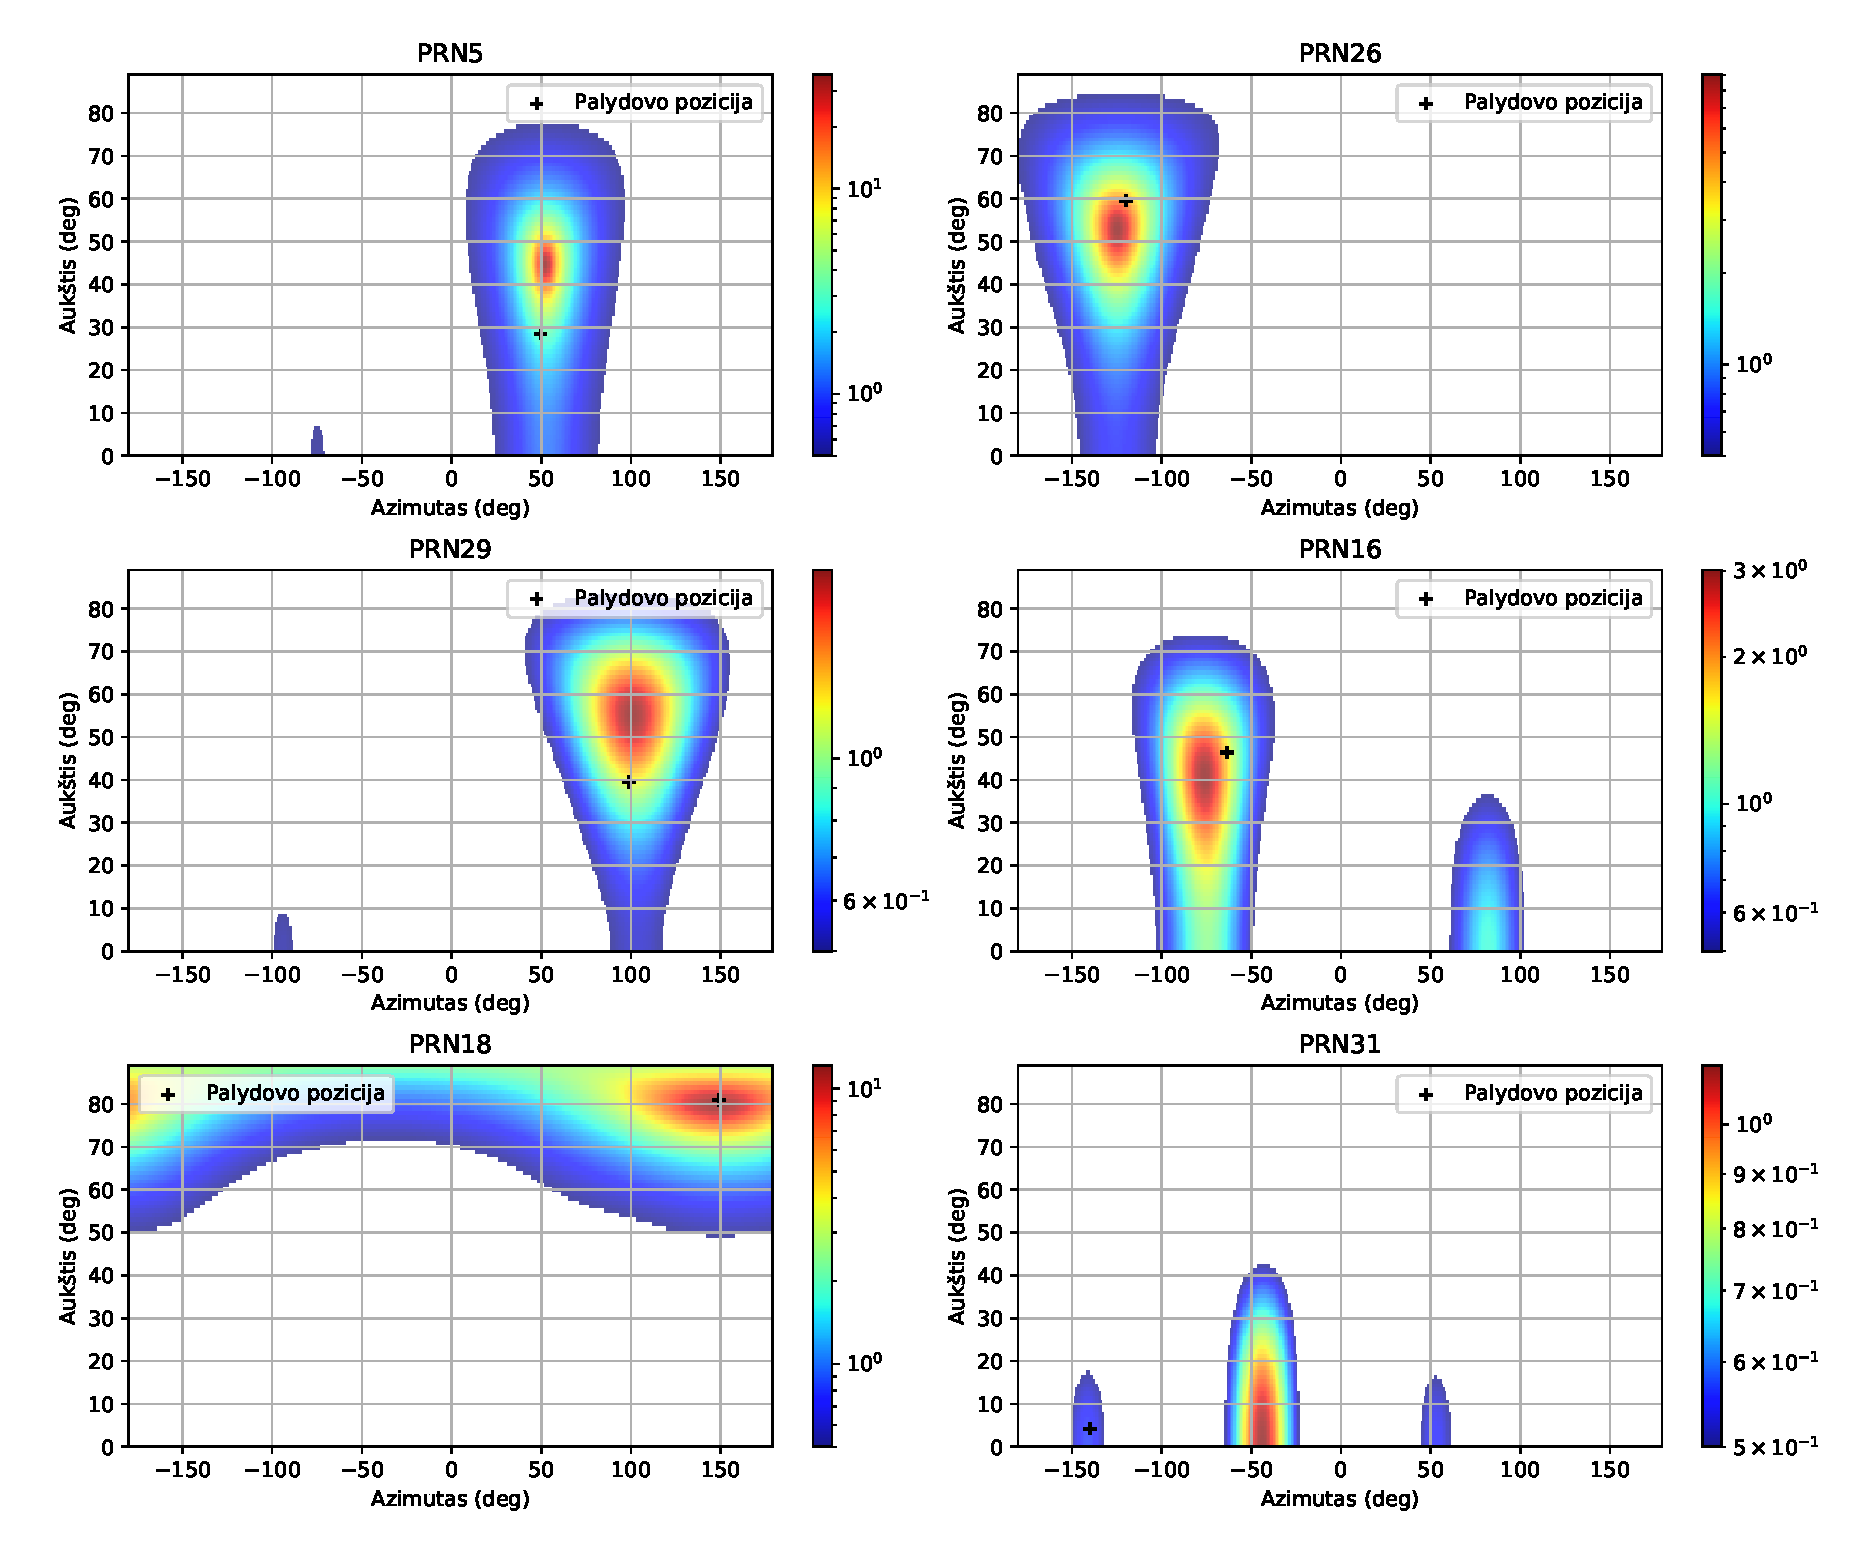
\includegraphics[scale=0.55]{drawings/no_reflection}
    \par\end{centering}
    \protect\caption{\label{fig:no_reflection}Nustatytos GPS palydovų signalų kryptys, naudojant MUSIC algoritmą.}
\end{figure}

\ref{fig:no_reflection_snr}~pav. pavaizduotas signalo triukšmo santykis, kiekvieno palydovo,
pritaikius spindulio formavimą aprašytą \ref{sec:beamforming_concept} skyriuje, o
signalo triukšmo santykis suskaičiuotas pagal \ref{sec:gnss_snr} skyriuje aprašytą
metodiką.

Spindulio formavimas atliekamas maksimumą nukreipiant į tikrąją palydovo padėti.
\ref{fig:no_reflection_snr}~pav. galima stebėti, kad naudojant spindulio formavimą,
signalo triukšmo santykis pagerėja nuo $2\ \mathrm{dB-Hz}$. iki $8\ \mathrm{dB-Hz}$.
Kadangi naudojamos 4 antenos, tai numatomas signalo pagerėjimas yra $6\ \mathrm{dB}$,
kas ir yra stebima signalo triukšmo santykio matavimuose. Taip pat PRN10 ir PRN27 atveju,
nenaudojant spindulio formavimo palydovo signalas buvo per silpnas, kad būtų
įmanoma vykdyti jo sekimą, todėl naudojant spindulio formavimą buvo aptikta
daugiau palydovų, kas leidžia tiksliau nustatyti imtuvo poziciją.

\begin{figure}[ht]
    \begin{centering}
    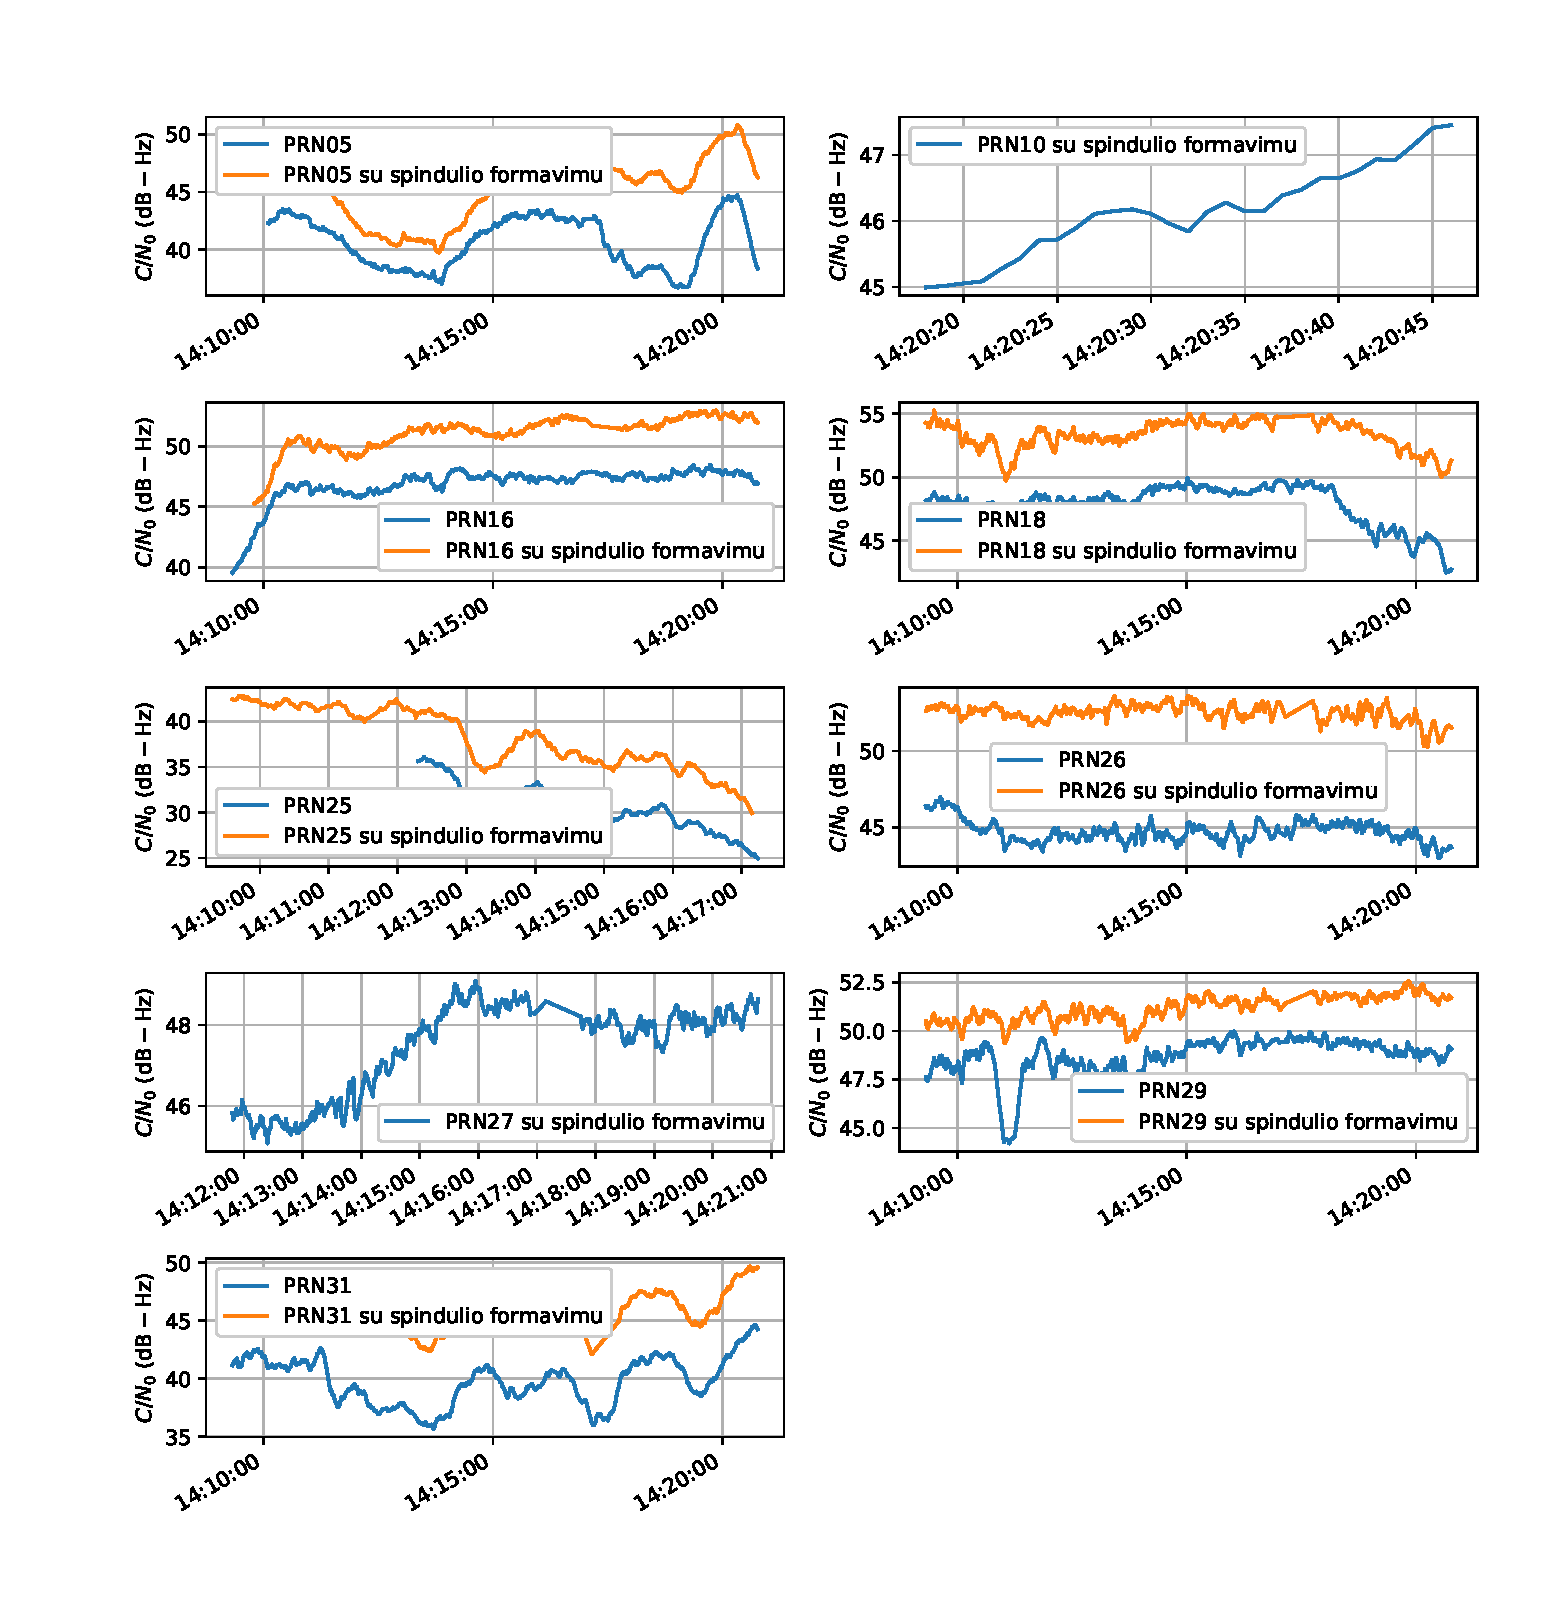
\includegraphics[scale=0.6]{drawings/no_refelection_snr}
    \par\end{centering}
    \protect\caption{\label{fig:no_reflection_snr}Nustatytas signalo triukšmo santykis nenaudojant ir naudojant spindulio formavimą.}
\end{figure}

Atlikus spindulio formavimą, suskaičiuotos koordinatės pavaizduotos \ref{fig:no_reflection_map}~pav.
Iš grafiko galime matyti, kad koordinatės taškų išsibarstymas truputį sumažėjo, tačiau reikšmingų
pokyčių nėra. Šį rezultatą pagrinde įtakoja geresnis signalo triukšmo santykis, bei atsiradę du papildomi
palydovai, kaip aptarta šio skyrelio pradžioje. Kadangi \ref{fig:no_reflection}~pav. atspindžių
nematome, tai šiam matavimui atspindžiai nesudarė papildomo trikdžio koordinačių skaičiavime.

\begin{figure}[ht]
    \begin{centering}
    \hspace*{-3cm}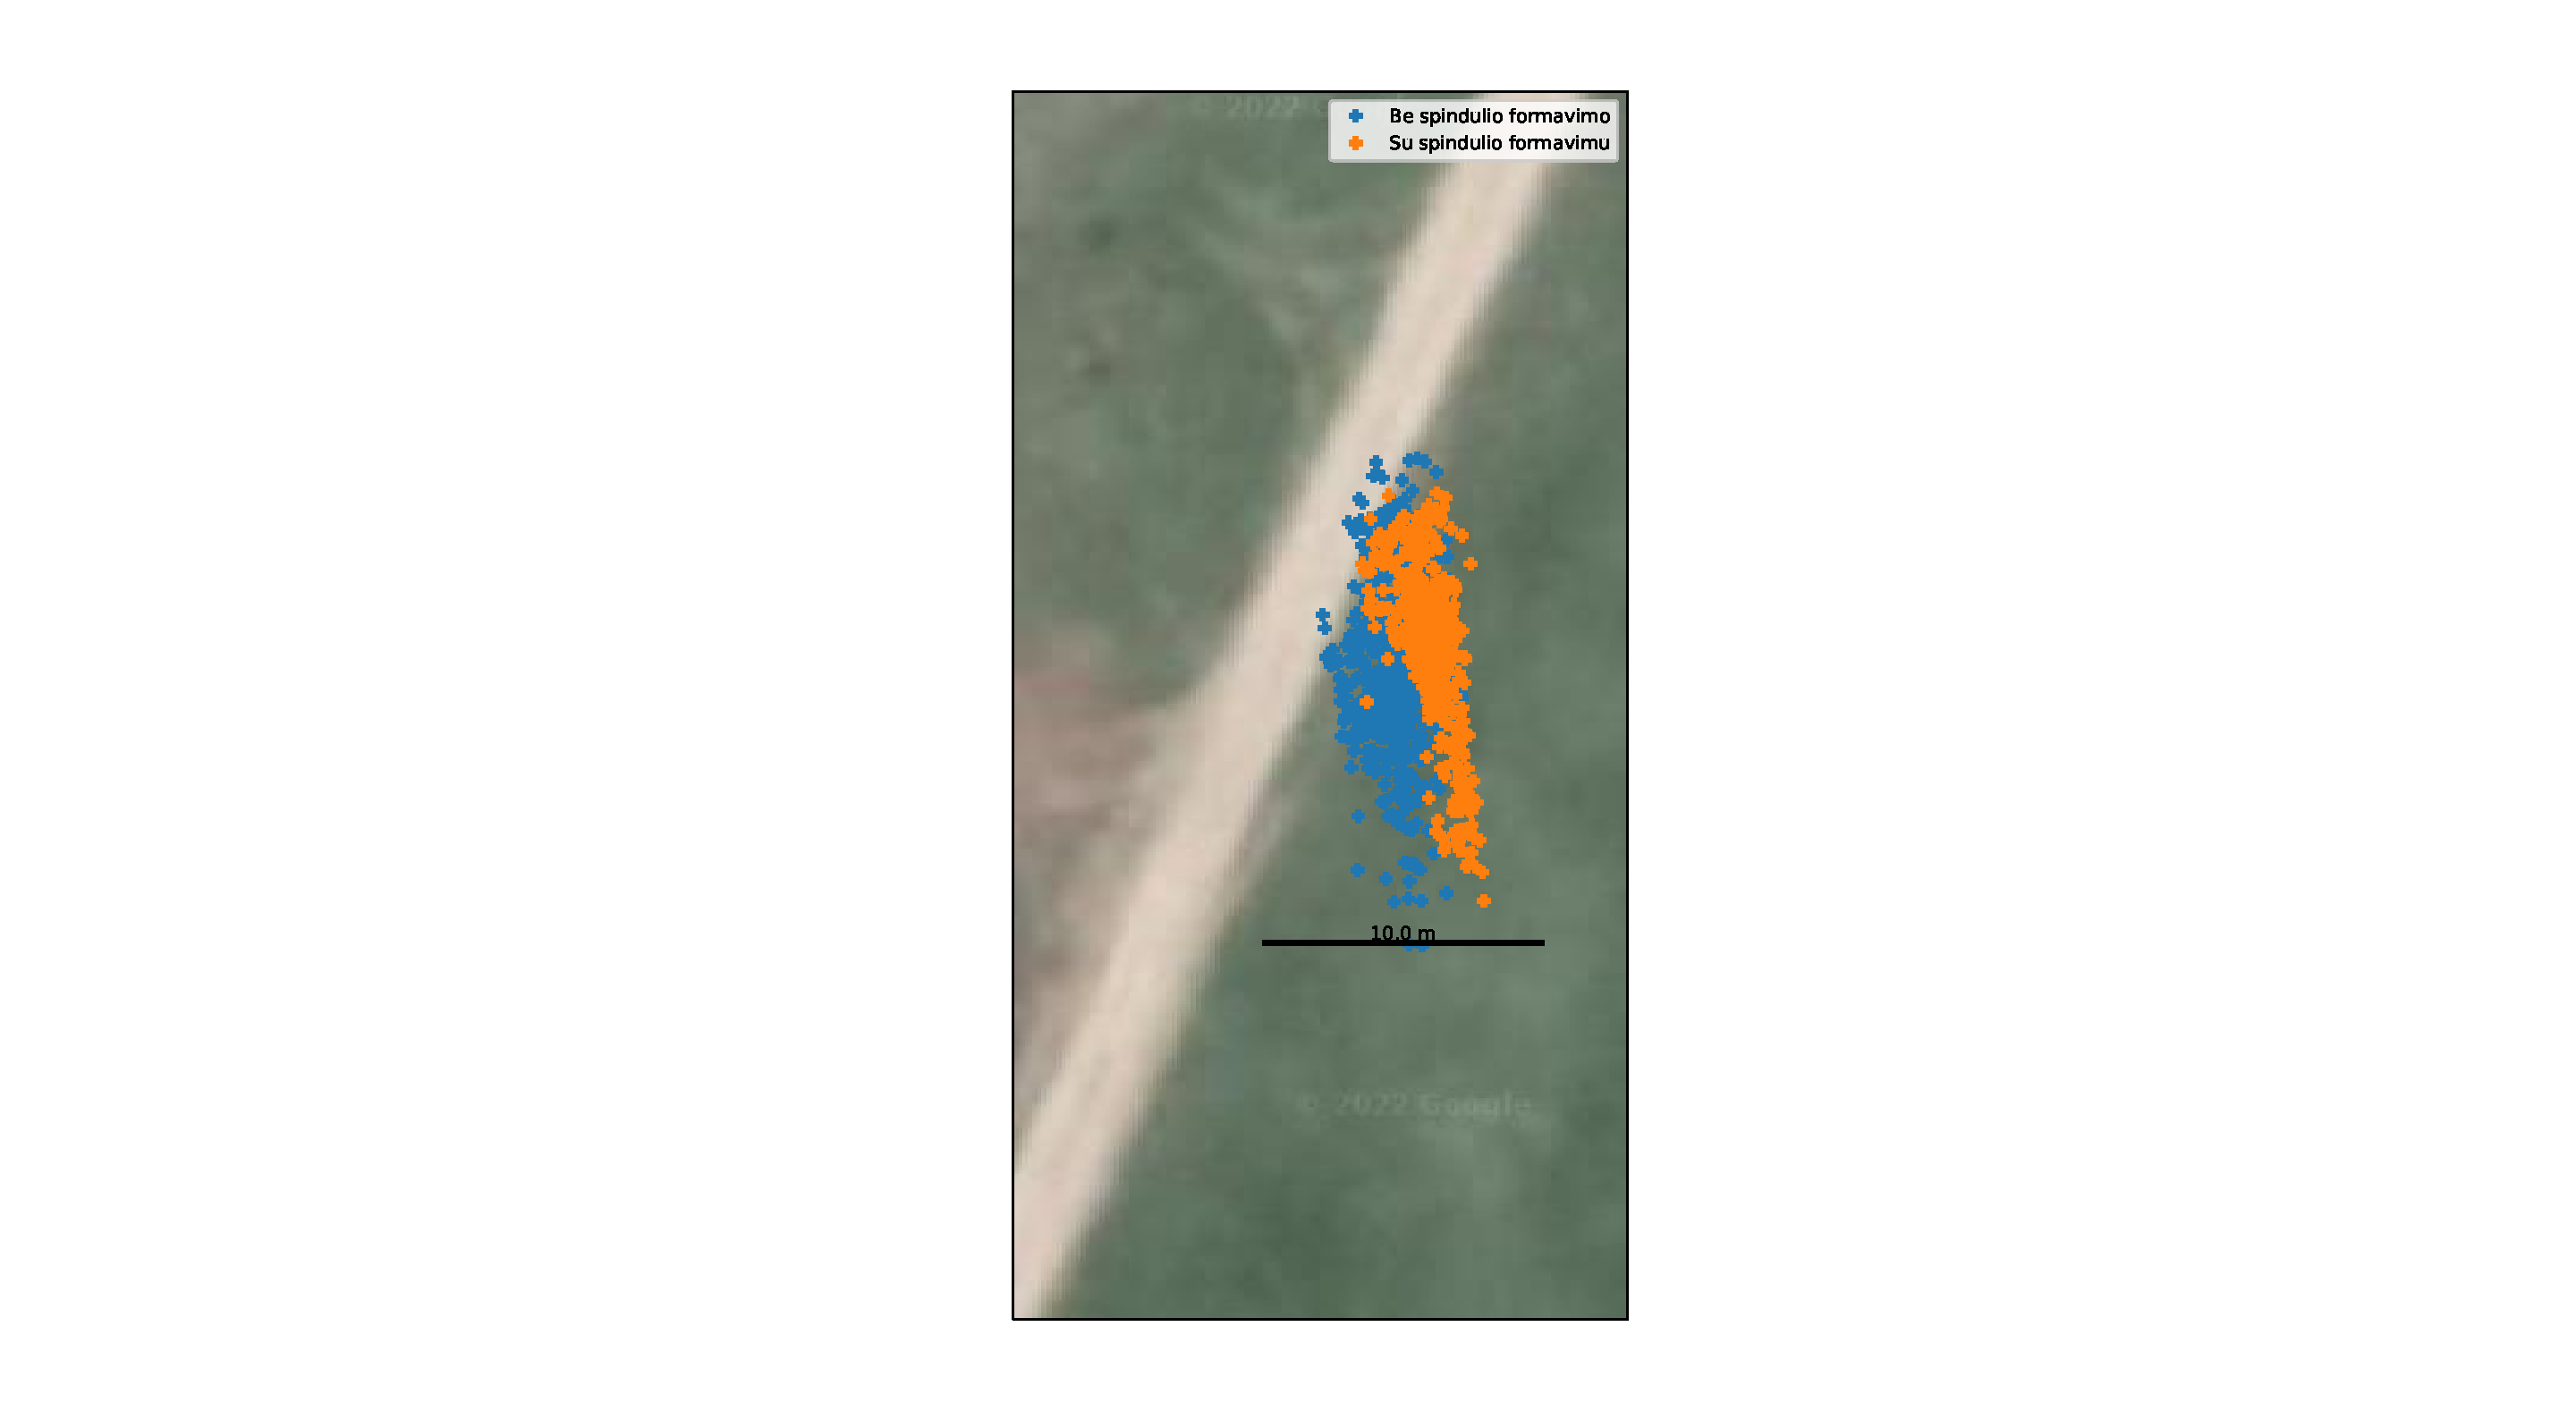
\includegraphics[scale=0.45]{drawings/no_reflection_map}
    \par\end{centering}
    \protect\caption{\label{fig:no_reflection_map}Imtuvo pozicijos koordinatės su spindulio formavimu ir be spindulio formavimo. Palydovinės nuotraukos \cite{google_maps}.}
\end{figure}



\subsubsection{GNSS signalų priėmimas kai atspindžiai vyksta nuo vieno pastato}\label{sec:gnss_meas_one_reflection}

Antras matavimas buvo daromas vietovėje kur yra vienas, nedidelis pastatas, nuo kurio gali atsirasti
signalo atspindžiai. Matavimo vieta ir laikas (palydovų išsidėstymas) pavaizduoti \ref{fig:two_reflection_sat_pos}~pav.
Vieta pasirinkta taip kad dalis dangaus skliauto būtų atviras, o kita dalis būtų blokuojama pastato.
palydovų išsidėstymas parinktas taip, kad jų signalas, kristu kuo statmeniau į pastato paviršių.
Palydovinėje nuotraukoje raudonu kryžiuku pažymėta apytikslė matavimų vieta. Raudonos rodykles
vaizduoja apytiksles palydovų signalų kryptis. Iš signalų krypčių, galime mėginti spėti,
kad atspindys bus matomas PRN21 ir PRN08 palydovų.

\begin{figure}[ht]
    \begin{centering}
    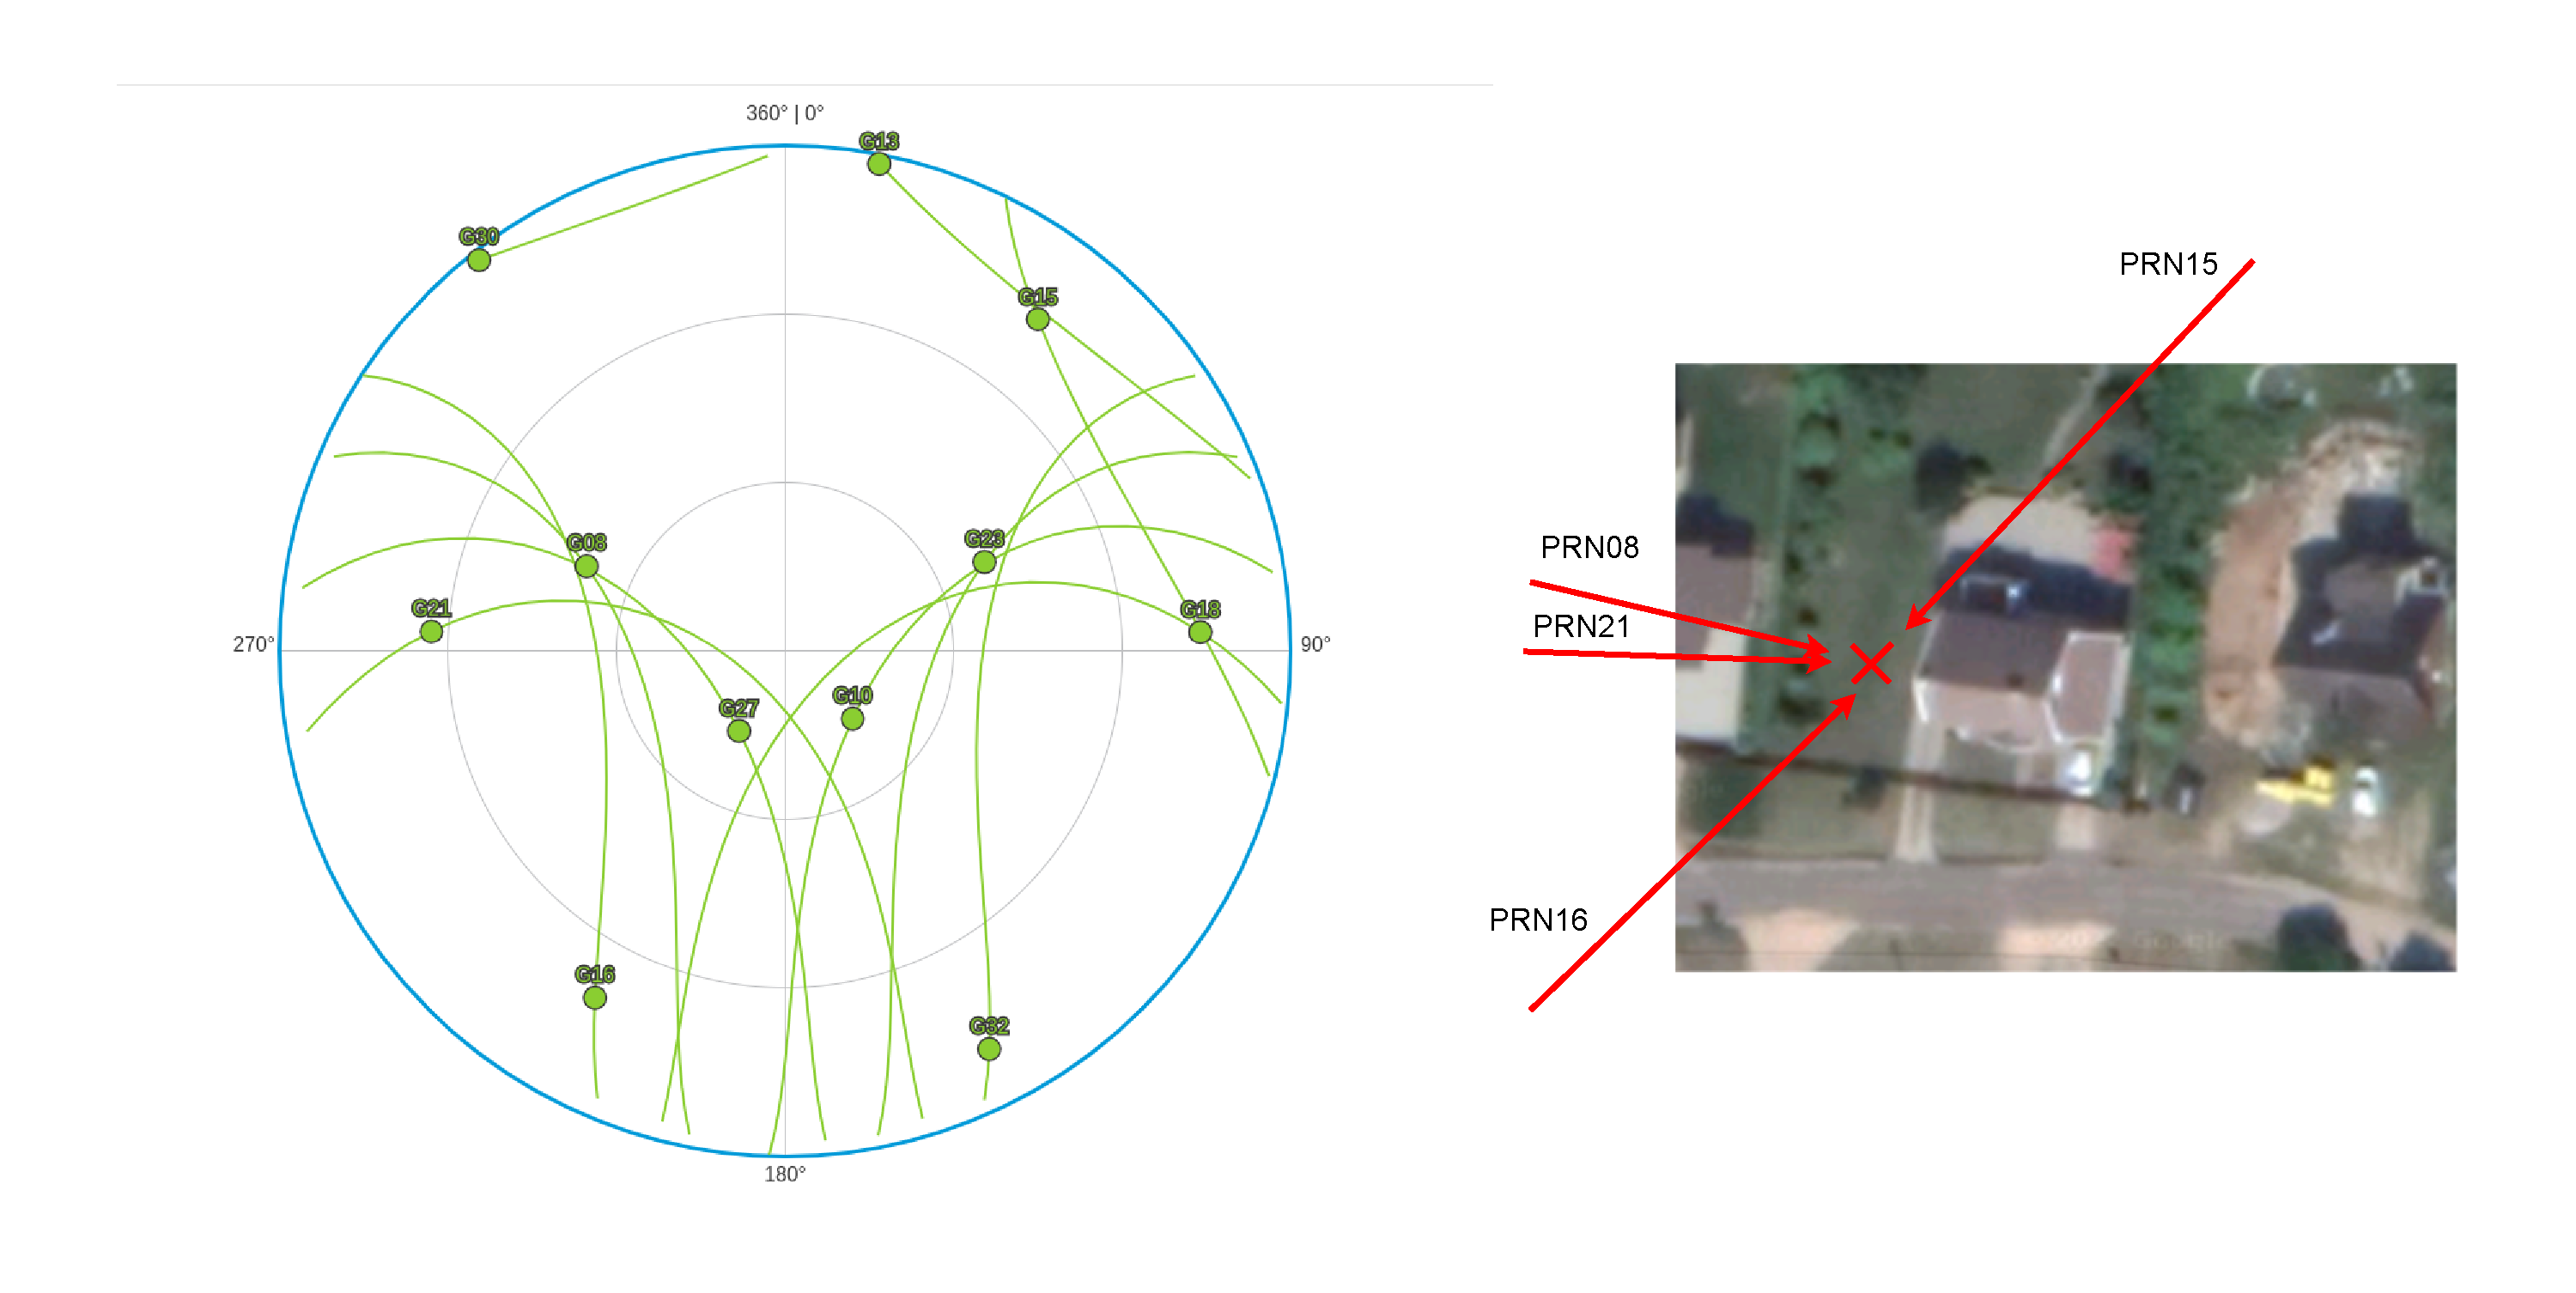
\includegraphics[scale=0.3]{drawings/one_reflection_sats.drawio}
    \par\end{centering}
    \protect\caption{\label{fig:single_reflection_sat_pos}Kairėje palydovų išsidėstymas dangaus skliaute matavimų metu, dešinėje matavimo vietovės palydovinė nuotrauka \cite{google_maps}.}
\end{figure}

\ref{fig:single_reflection}~pav. pavaizduotas MUSIC algoritmo pseudospektro vertės. Grafikų
fonas yra panoraminė nuotrauka, kuri buvo padaryta matavimo vietoje. Nuotrauka yra sukalibruota pagal
pastato aukštį ir apytiksles pasaulio šalis. Grafike dauguma palydovų turi vieną,
aiškų maksimumą, tačiau PRN08 turi du maksimumus: vieną labai stiprų ir kitą silpnesnį.
PRN21 turi 2 beveik identiškus maksimumus.
Abiem atvejais stipresnės pseudospektro vertės yra stebimos tiesiogiai atėjusio signalo, tačiau
matomas ir atspindys nuo šalia esančio pastato. Iš šių matavimų matome, kad vyksta atspindžiai
nuo pastato ir tai galimai sukelią trukdį koordinačių skaičiavime.
Kitų palydovų signalai beveik sutampa su tikrosiomis palydovų padėtimis, tačiau dėl priežasčių aptartų
\ref{sec:gnss_meas_no_reflection} skyriuje, maksimumai tiksliai nesutampa su tikrosiomis palydovų padėtimis.

\begin{figure}[ht]
    \begin{centering}
    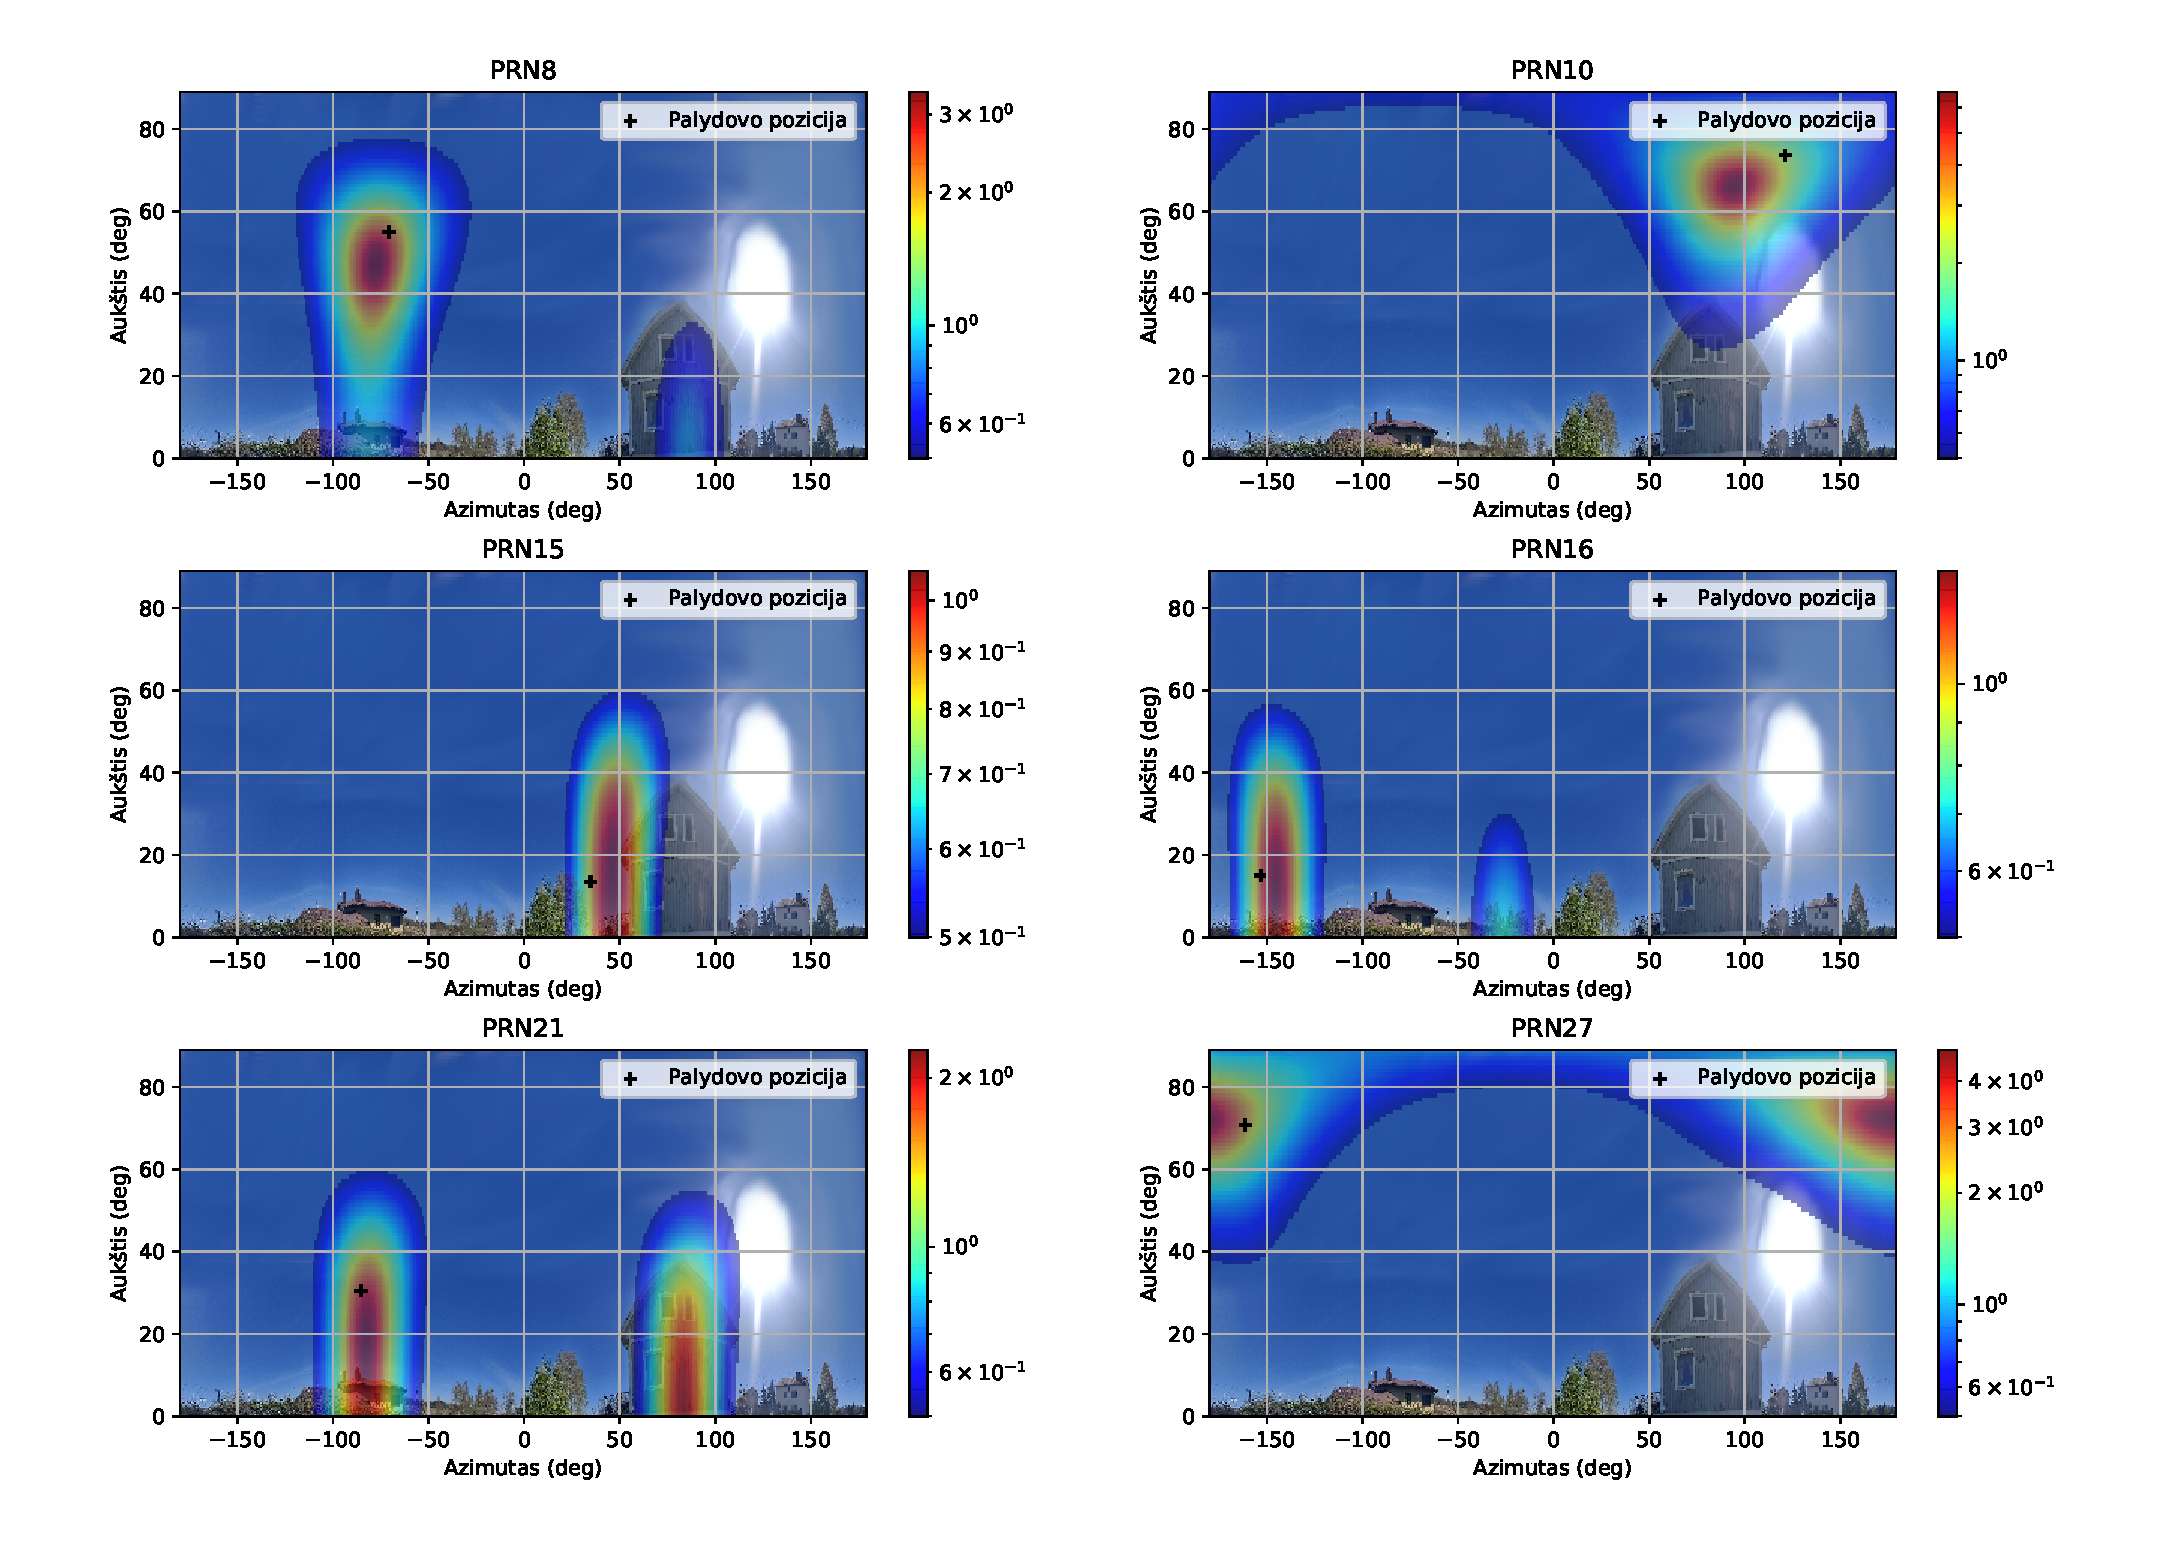
\includegraphics[scale=0.45]{drawings/one_reflection_2}
    \par\end{centering}
    \protect\caption{\label{fig:single_reflection}Nustatytos GPS palydovų signalų kryptys, naudojant MUSIC algoritmą.}
\end{figure}

\ref{fig:single_reflection_snr}~pav. pavaizduotas signalo triukšmo santykis atliekant spindulio formavimą,
maksimumą nutaikant į tikrąją palydovo padėtį. Kaip ir pirmojo matavimo atveju, stebimas signalo triukšmo
santykio padidėjimas
nuo $2\ \mathrm{dB-Hz}$ iki $8\ \mathrm{dB-Hz}$. Kaip ir pirmuoju atveju,
imtuvas priima signalą iš vieno papildomo palydovo, kai vykdomas spindulio formavimas.

\begin{figure}[ht]
    \begin{centering}
    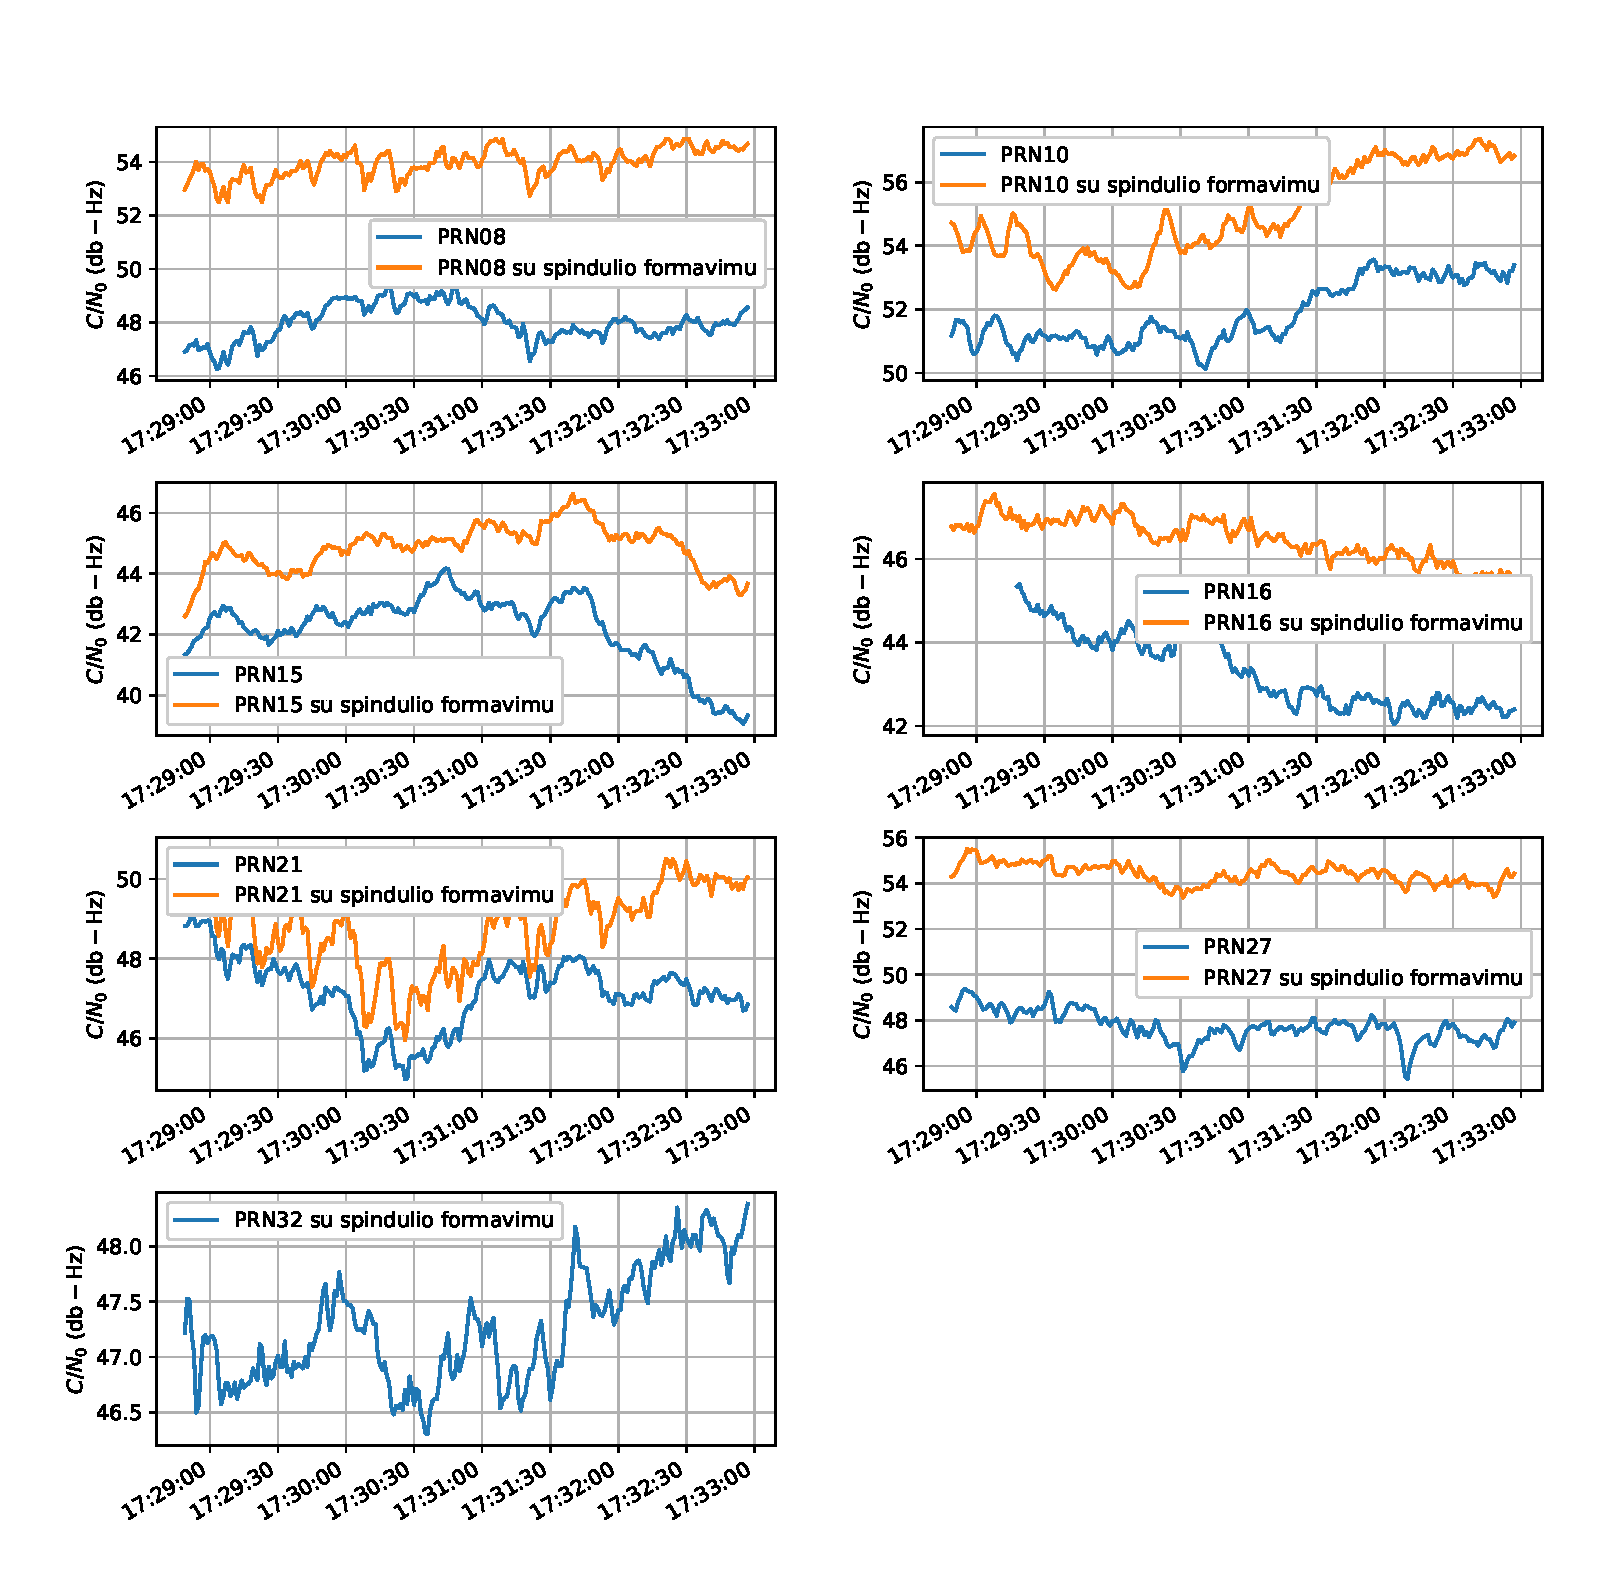
\includegraphics[scale=0.6]{drawings/one_reflection_snr}
    \par\end{centering}
    \protect\caption{\label{fig:single_reflection_snr}Nustatytas signalo triukšmo santykis nenaudojant ir naudojant spindulio formavimą.}
\end{figure}

Iš \ref{fig:single_reflection_map}~pav. galime nustatyti, kad koordinačių nuokrypis sumažėjo taikant spindulio
formavimą, bei vidutinė koordinatė pasistūmė toliau nuo pastato. Iš vidutinės koordinatės pokyčio
galime daryti išvadą, kad taikant spindulio formavimą, buvo nuslopintas atspindys. Esant atspindžiui,
koordinatė priartėja prie pastato, kadangi signalo kelias atsispindint nuo pastato pailgėja, dingus
atspindžiui signalo kelias sutrumpėja ir imtuvo koordinate gaunama esanti arčiau palydovo.
Koordinačių nuokrypis sumažėja ir dėl vieno papildomo palydovo.


\begin{figure}[ht]
    \begin{centering}
    \hspace*{-4cm}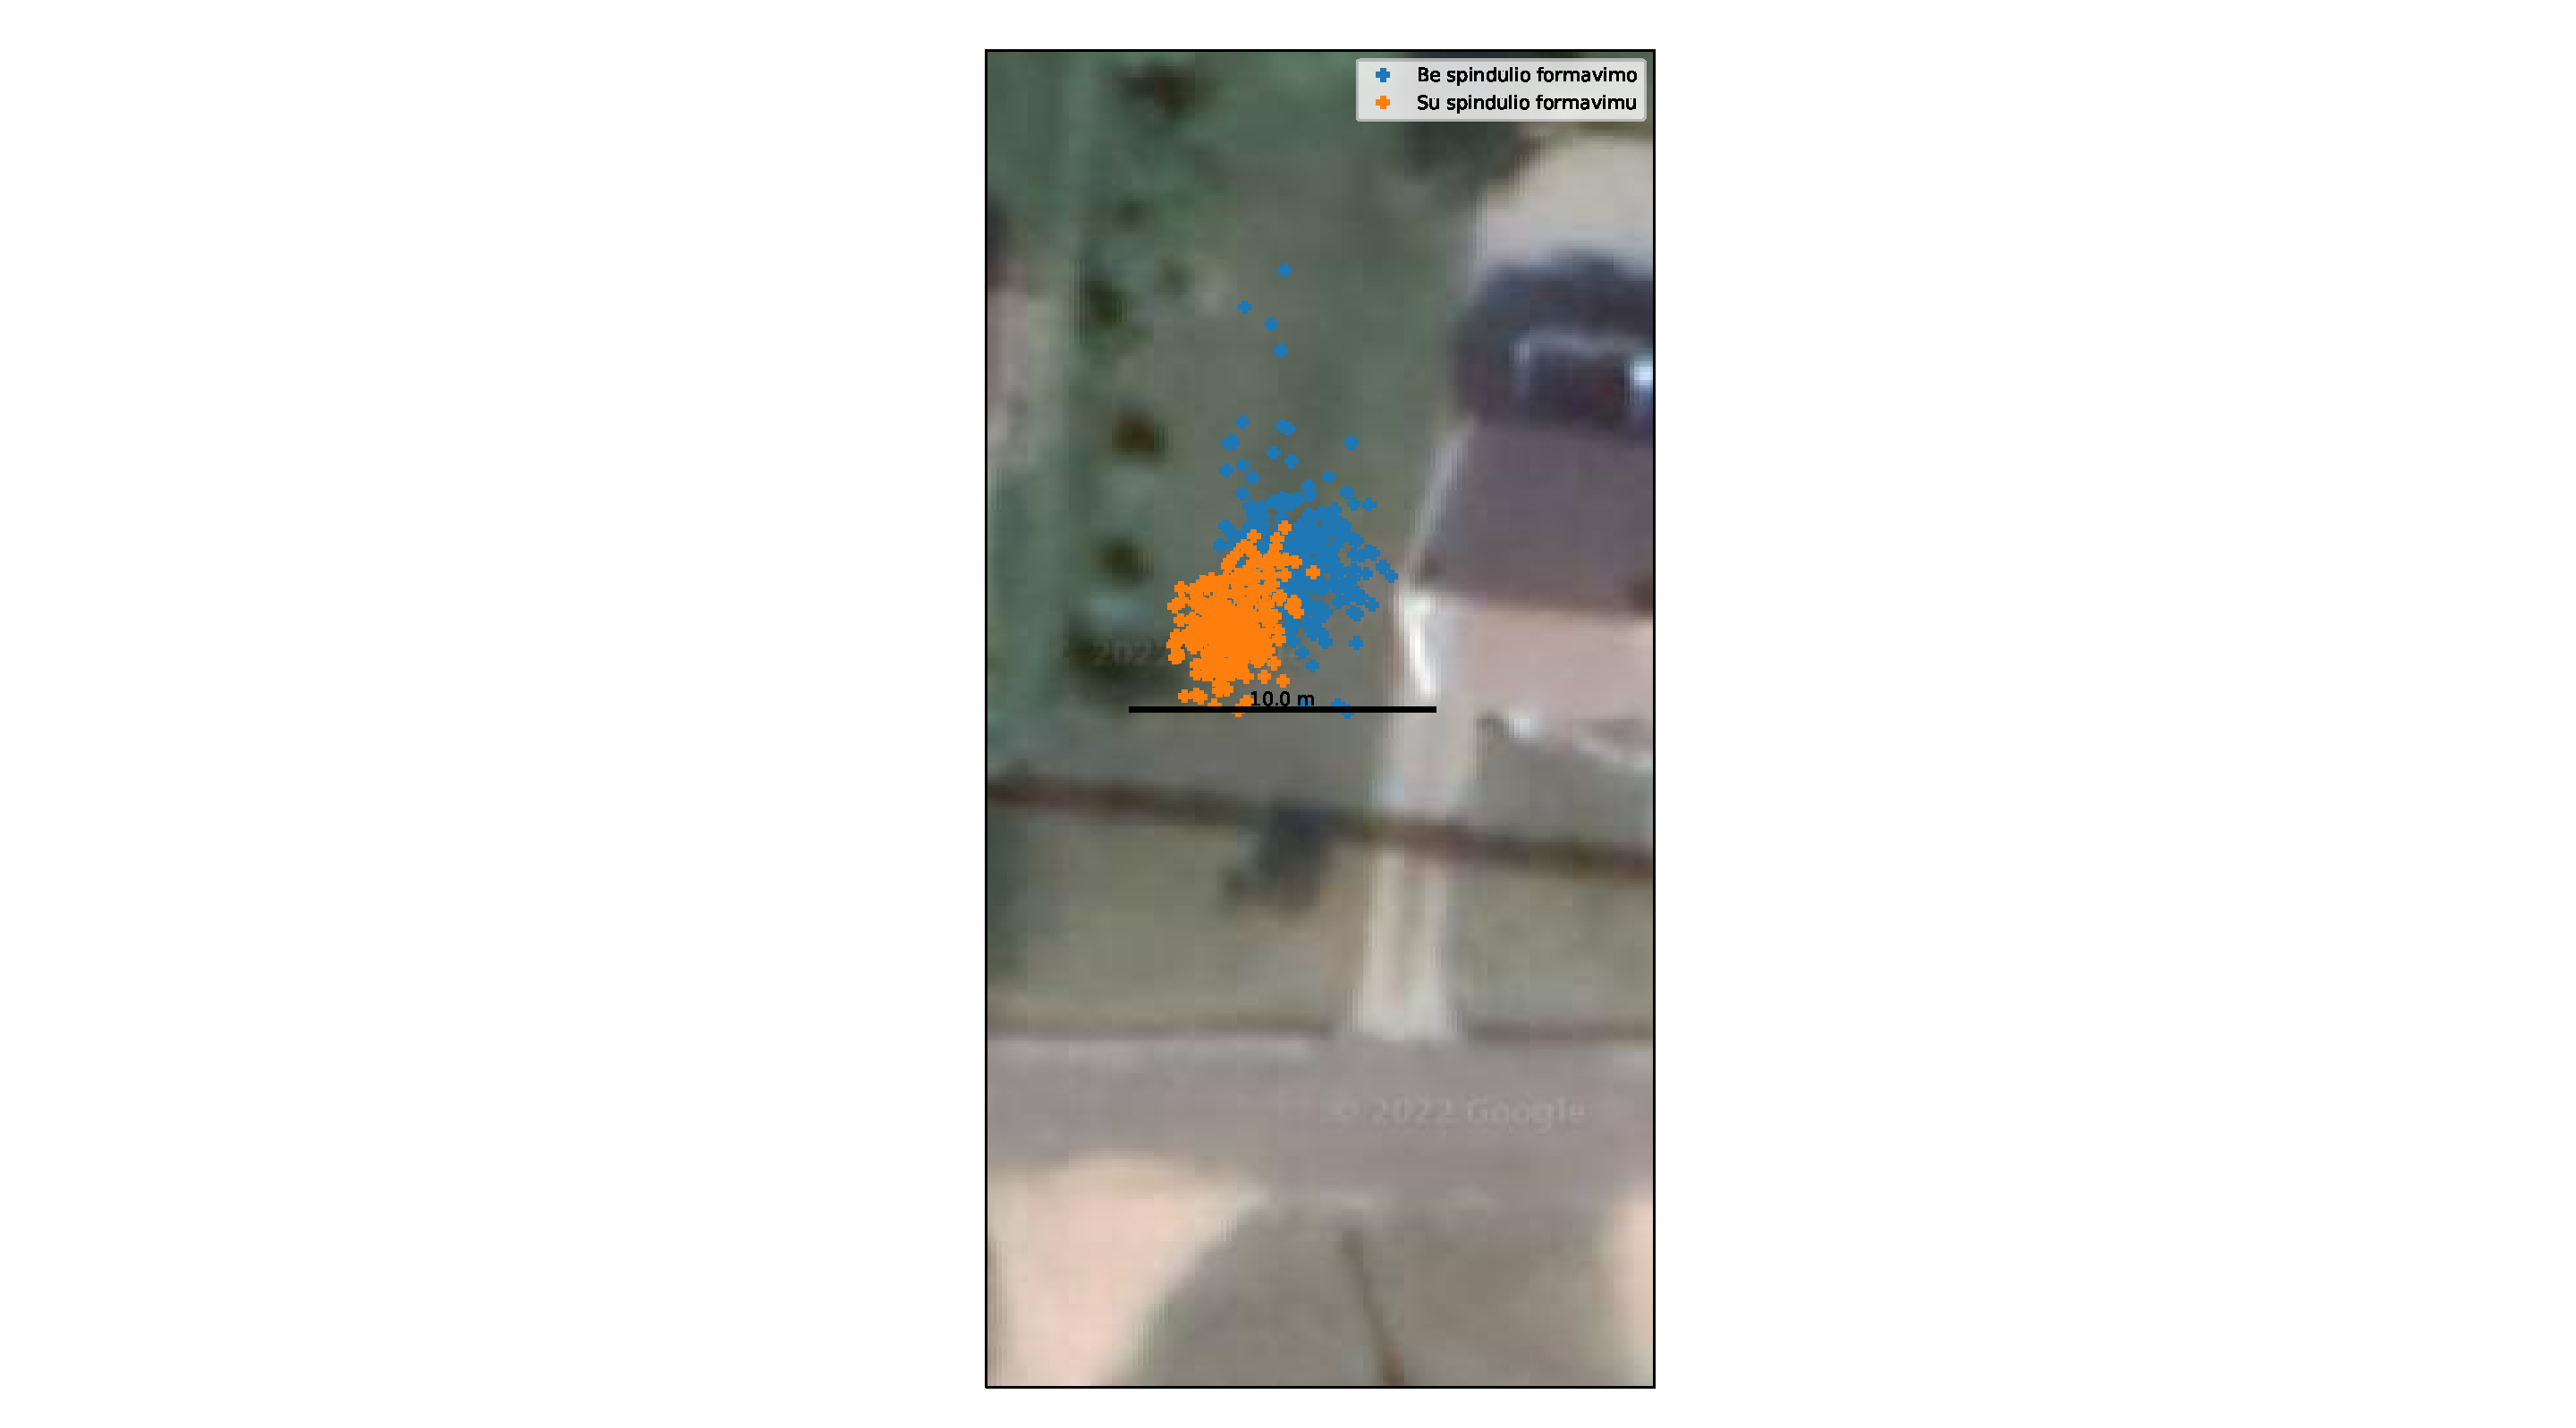
\includegraphics[scale=0.5]{drawings/one_reflection_map}
    \par\end{centering}
    \protect\caption{\label{fig:single_reflection_map}Imtuvo pozicijos koordinatės su spindulio formavimu ir be spindulio formavimo. Palydovinės nuotraukos \cite{google_maps}.}
\end{figure}

\subsubsection{GNSS signalų priėmimas urbanistinėje aplinkoje}\label{sec:gnss_meas_two_reflection}

Trečiajam matavimui pasirinkta vieta su dviem aukštais pastatais.
\ref{fig:two_reflection_sat_pos}~pav. raudonu kryžiuku pažymėta apytikslė matavimų
vieta. Rytuose ir vakaruose yra du aukšti pastatai, kurie blokuoja tiesioginį signalą. 
\ref{fig:two_reflection_sat_pos}~pav. kairėje pavaizduotas palydovų išsidėstymas
matavimo metu, juodumomis rodyklėmis pažymėta palydovų judėjimo kryptis.

\begin{figure}[ht]
    \begin{centering}
    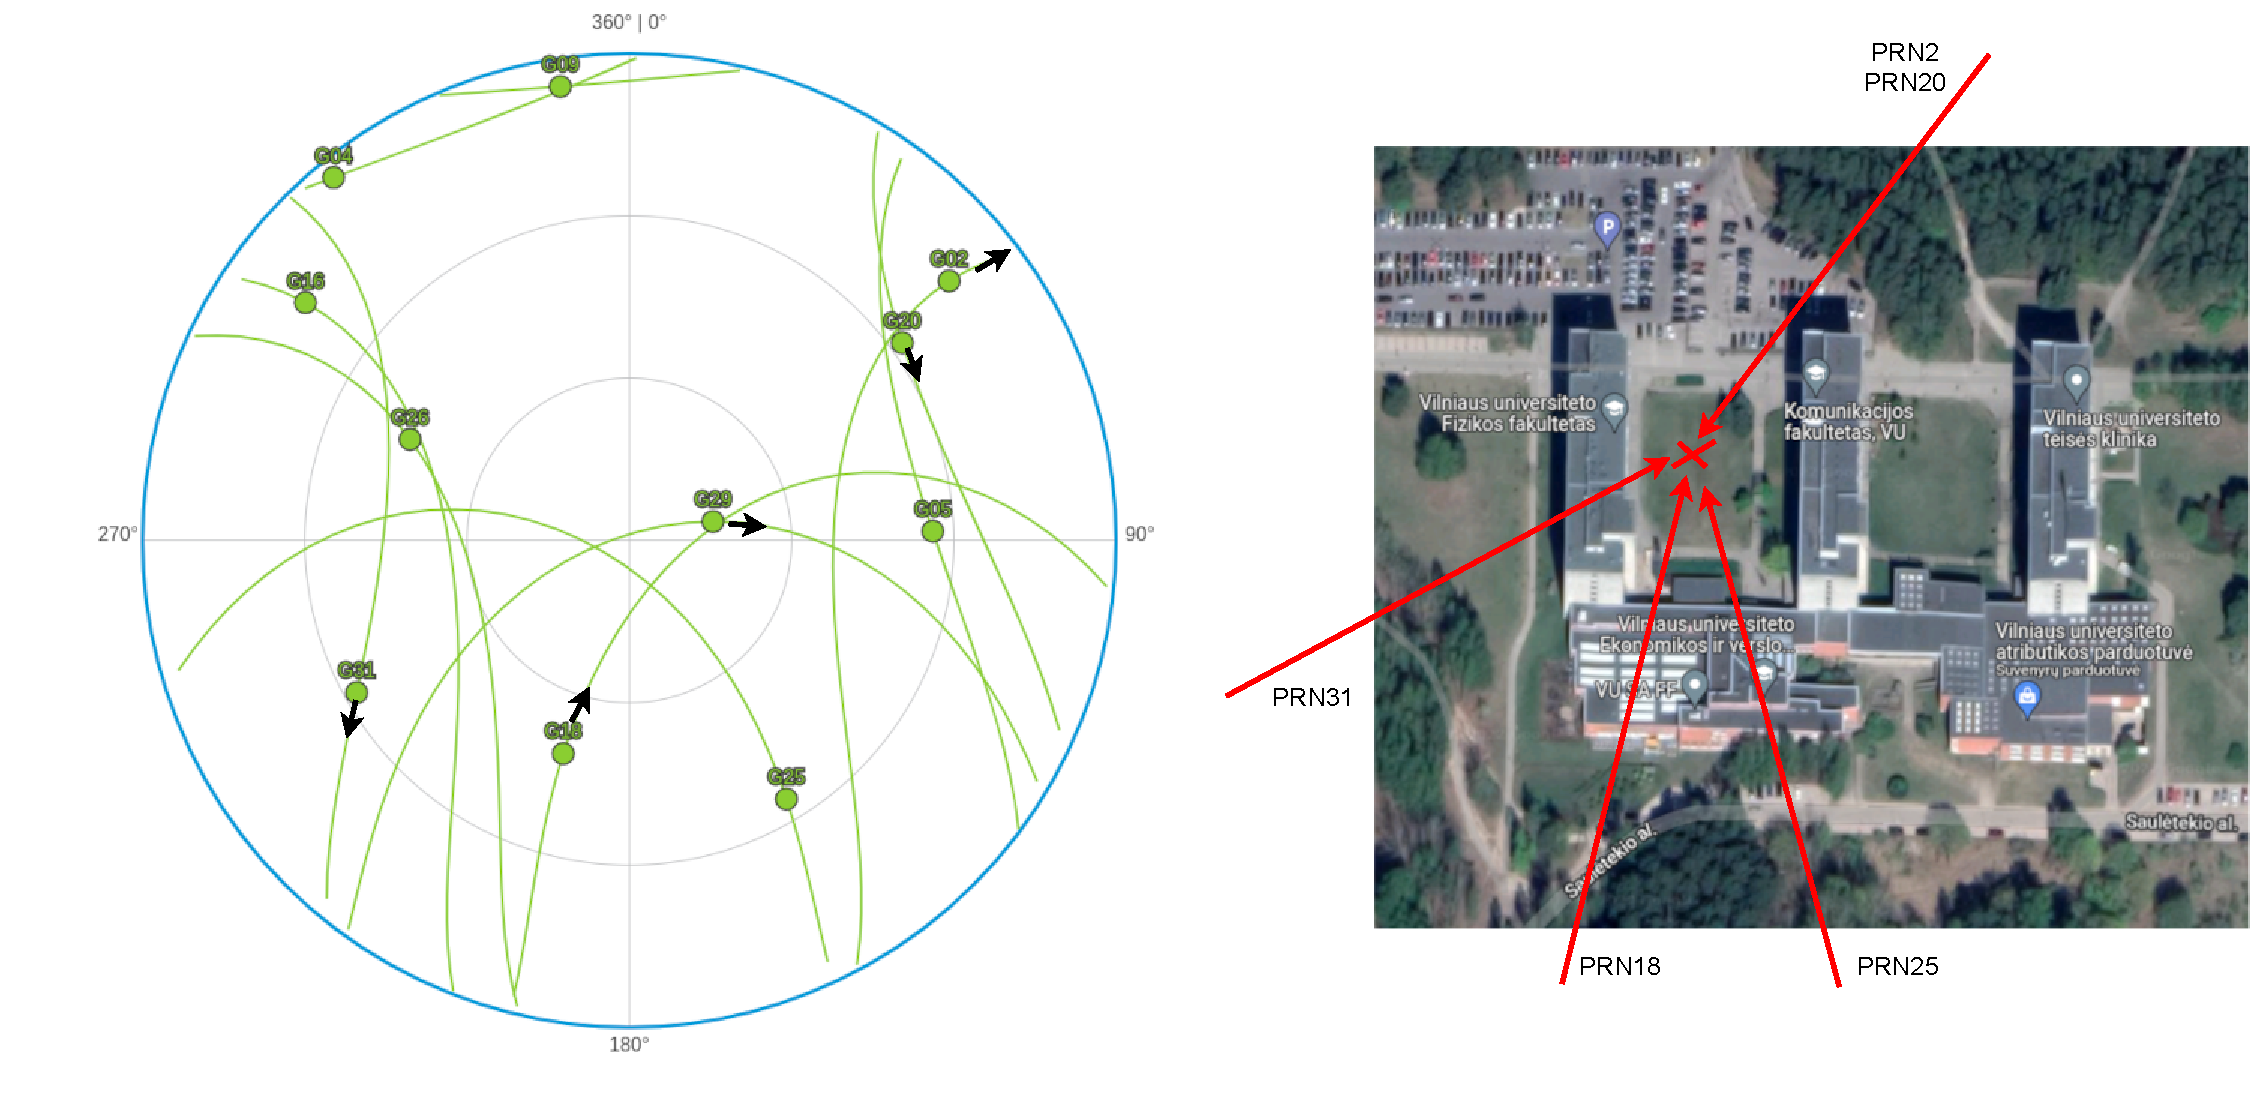
\includegraphics[scale=0.4]{drawings/vu_sats_map.drawio}
    \par\end{centering}
    \protect\caption{\label{fig:two_reflection_sat_pos}Kairėje palydovų išsidėstymas dangaus skliaute matavimų metu, dešinėje matavimo vietovės palydovinė nuotrauka \cite{google_maps}.}
\end{figure}

\ref{fig:two_reflection}~pav. pavaizduota nustatytos palydovų signalų kryptis.
Panoraminėje nuotraukoje matome, kad rytuose ir vakaruose yra du aukšti pastatai.
PRN2 galime matyti, kad signalas gaunamas tiesioginis, bet iš
\ref{fig:two_reflection_sat_pos}~pav. galime matyti, kad palydovas netrukus
pasislėps už pastato. Taip pat stebime nestiprų atspindį nuo pastato vakaruose
(apie $-60$ laipsnių). PRN31 palydovo atveju, tikroji padėtis yra apie $-120$
laipsnių kryptimi, bet čia joks signalas nestebimas, tačiau imtuvas stebi stiprų
atspindį nuo pastato rytuose.

\begin{figure}[ht]
    \begin{centering}
    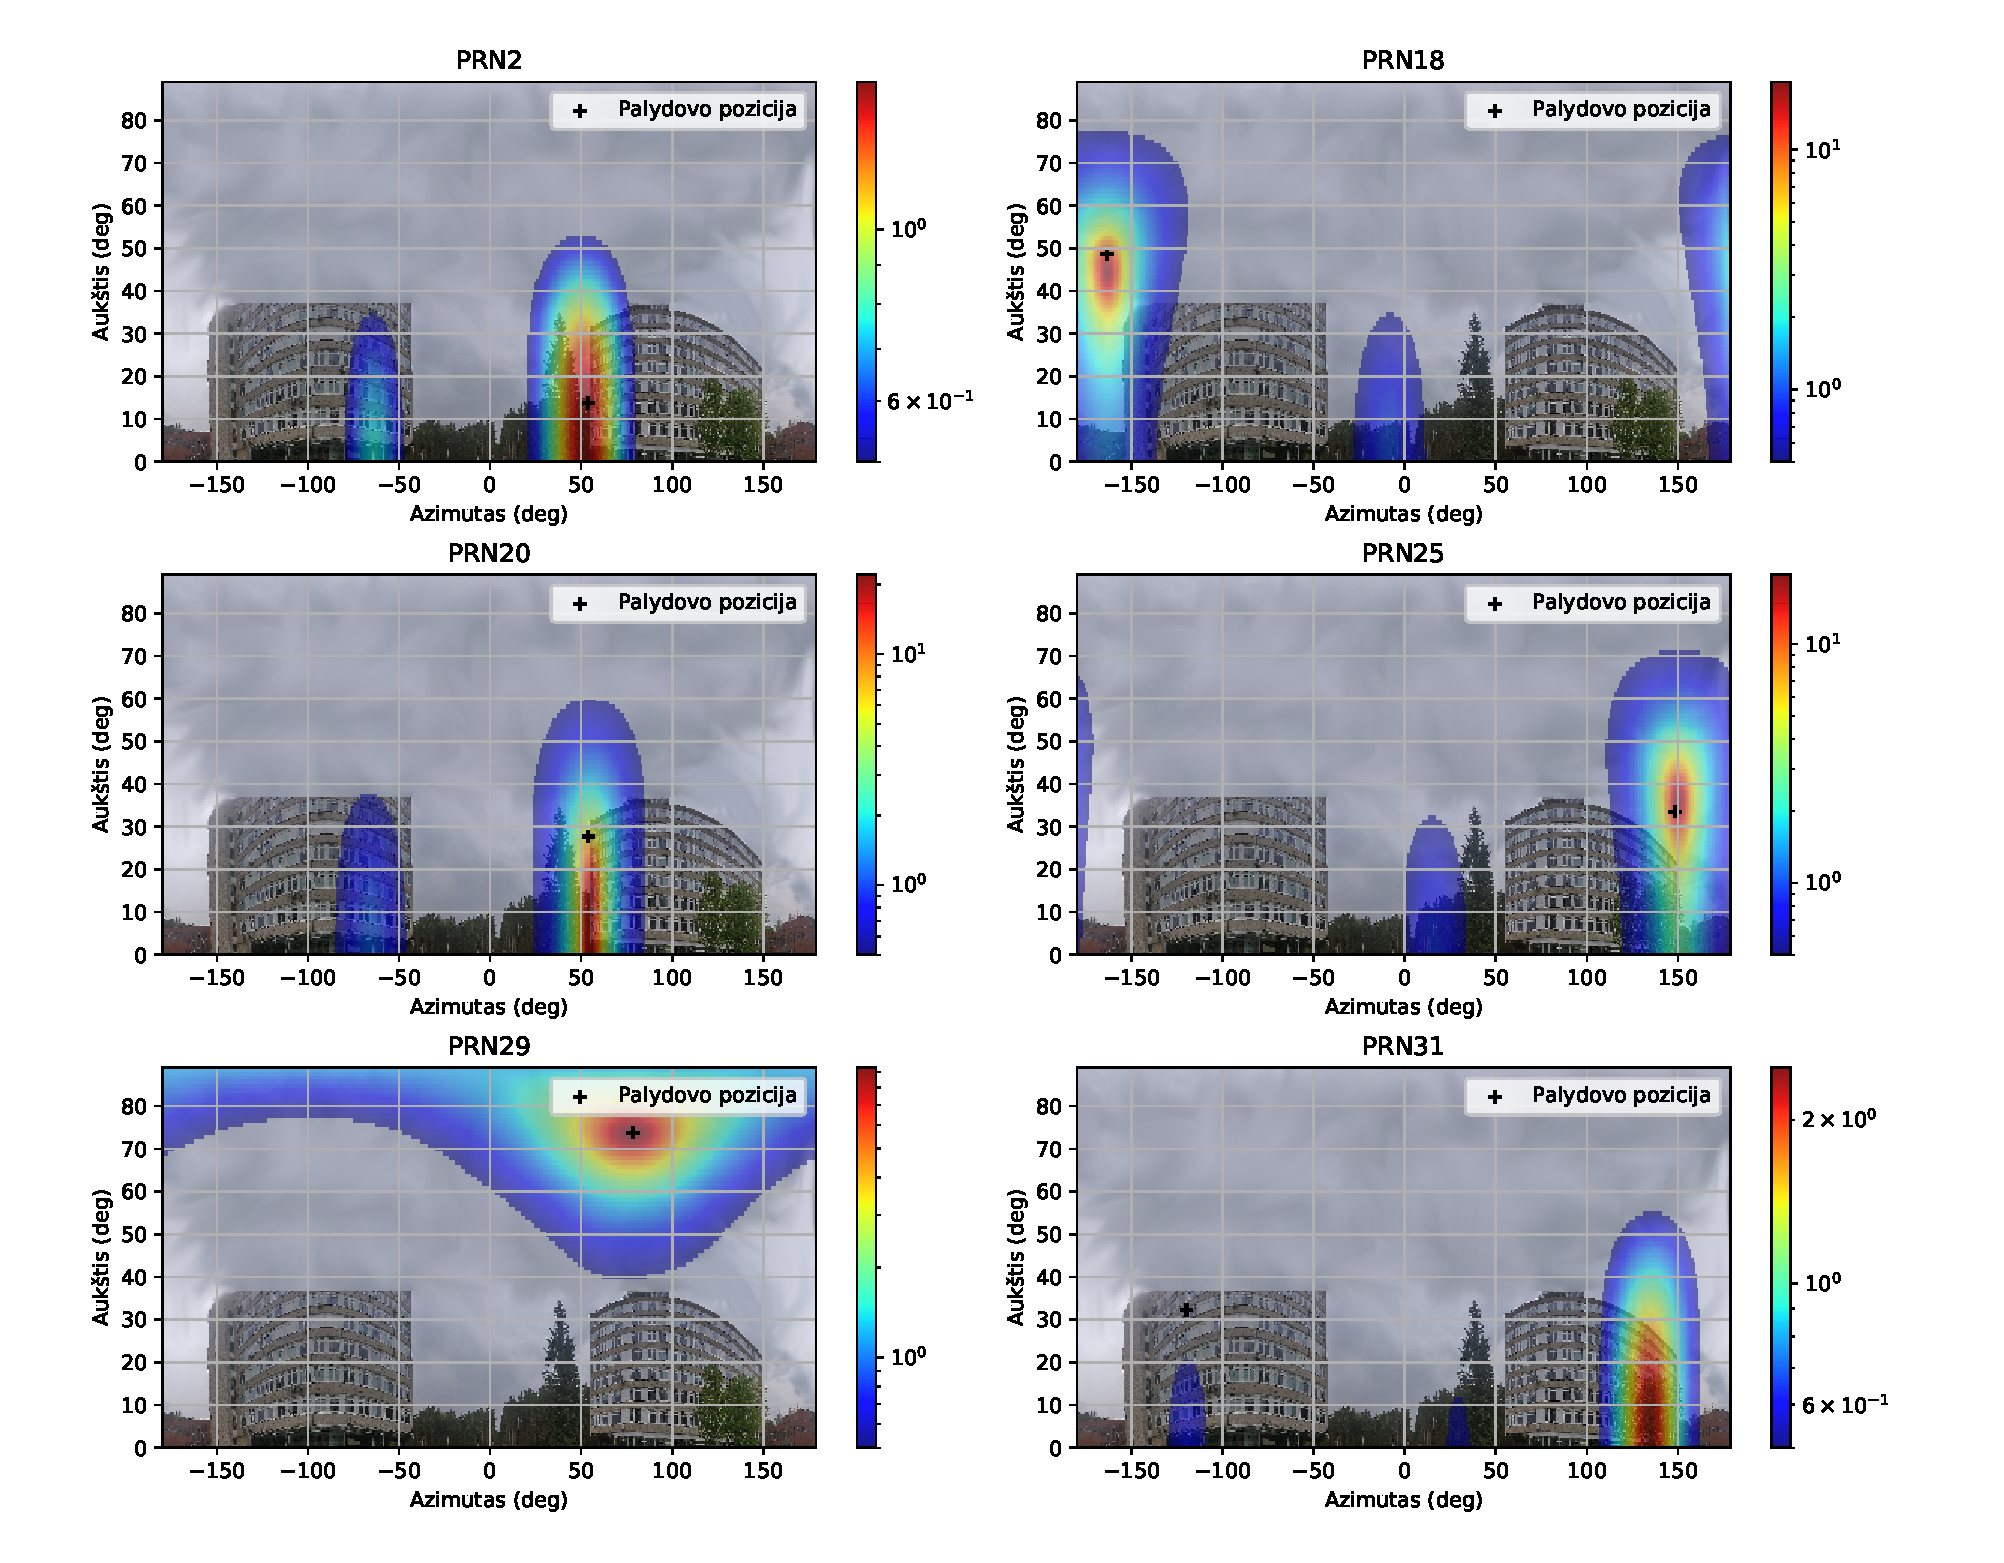
\includegraphics[scale=0.50]{drawings/two_reflections}
    \par\end{centering}
    \protect\caption{\label{fig:two_reflection}Nustatytos GPS palydovų signalų kryptys, naudojant MUSIC algoritmą.}
\end{figure}

\ref{fig:two_reflection_snr}~pav. pavaizduotas signalo triukšmo santykis su spindulio
ir be spindulio formavimo.  PRN02 atveju, po 5 minučių matavimo, galime
matyti, kad su spindulio formavimu,
signalo triukšmo santykis staigiai pradeda mažėti. Kaip aprašyta anksčiau, palydovas
pasislepia už pastato. Be spindulio formavimo PRN2 signale galime
stebėti signalo sumažėjimą, bet jis visiškai neišnyksta, kadangi
vietoje tiesioginio signalo, imtuvas pradeda matyti atspindį nuo pastato vakaruose.
PRN31 atveju su spindulio formavimu, iš pradžių signalas yra matomas, tačiau palydovui
leidžiantis, signalas pradingsta, pasislepia už pastato esančio vakaruose.

\begin{figure}[ht]
    \begin{centering}
    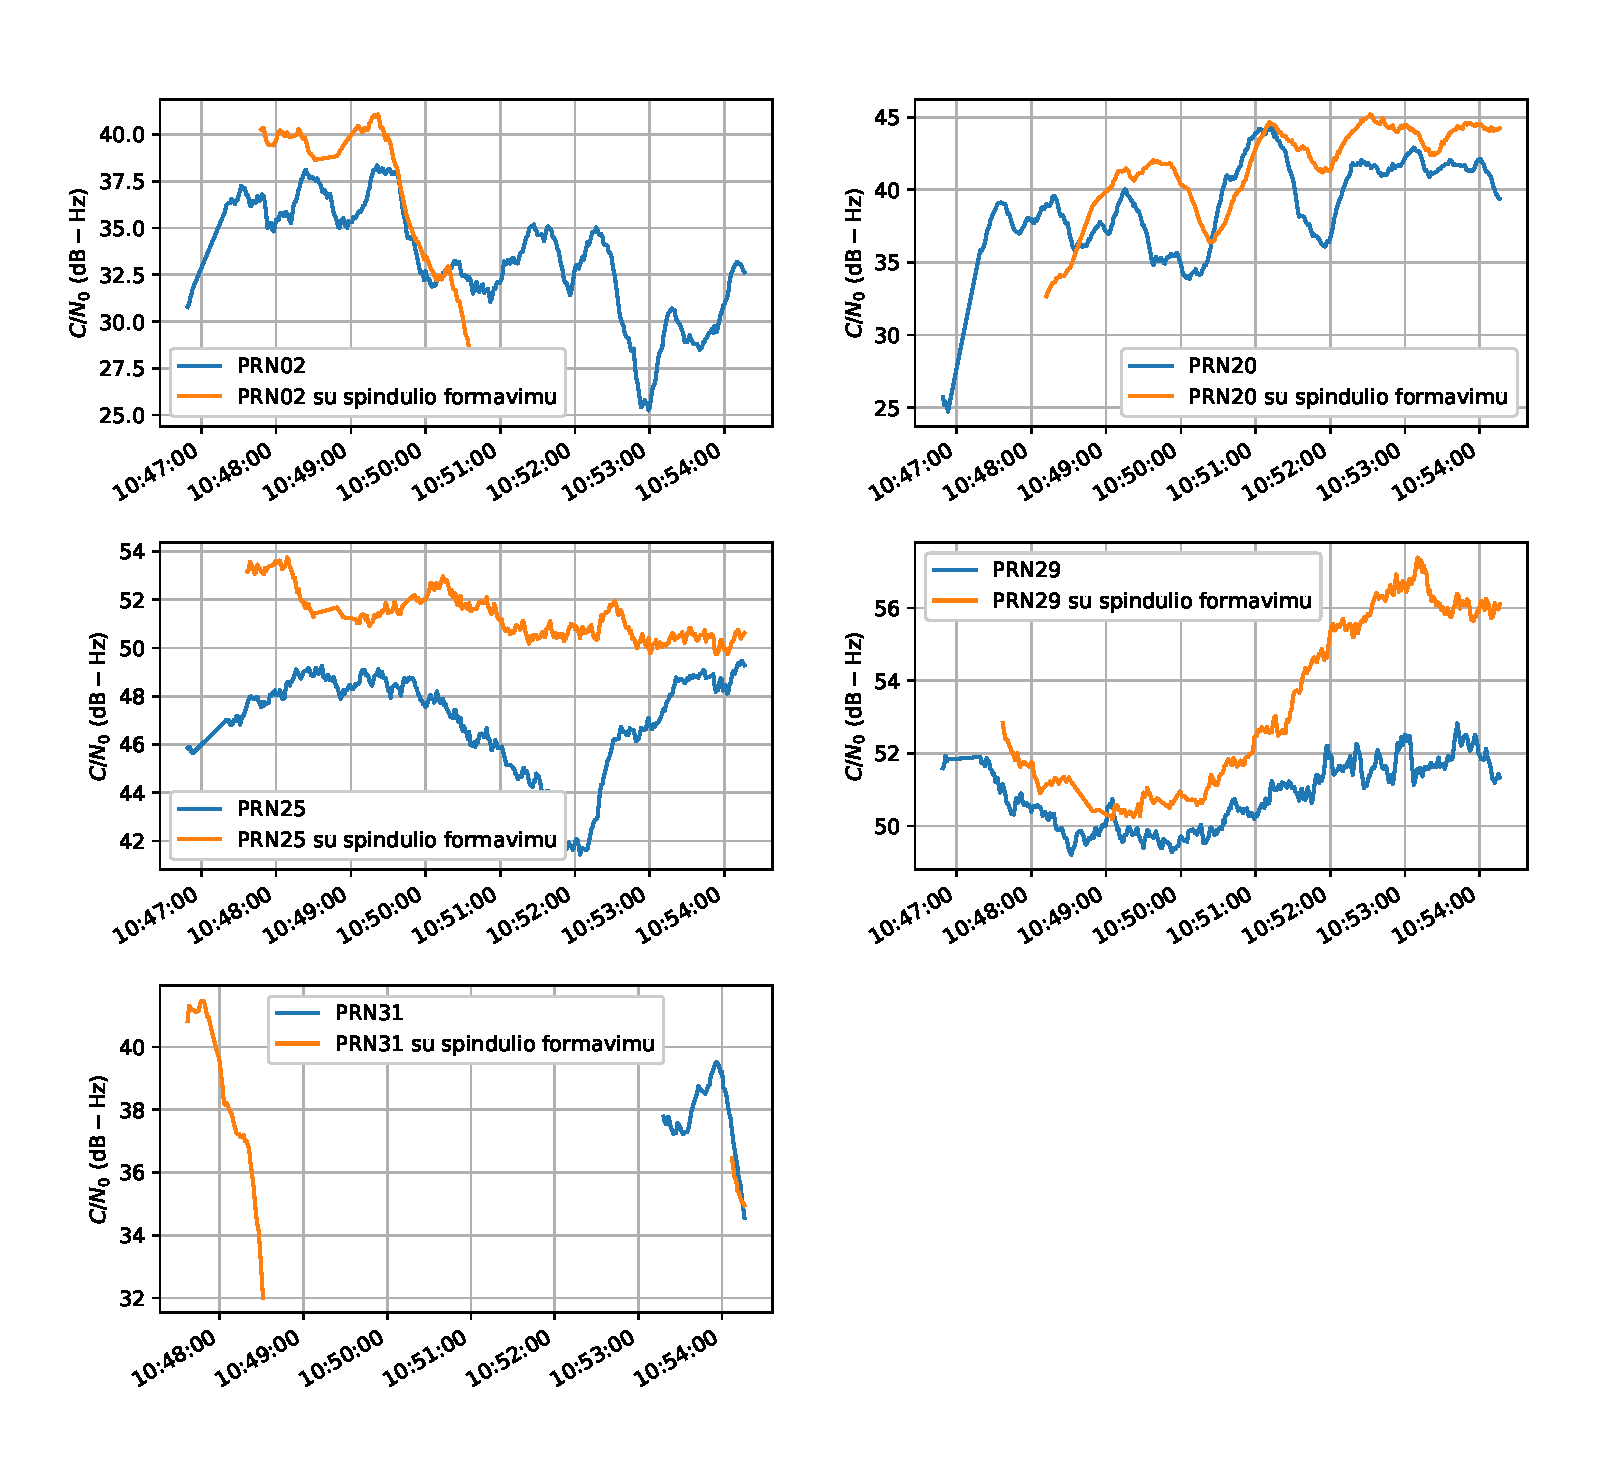
\includegraphics[scale=0.6]{drawings/two_reflections_snr}
    \par\end{centering}
    \protect\caption{\label{fig:two_reflection_snr}Nustatytas signalo triukšmo santykis nenaudojant ir naudojant spindulio formavimą.}
\end{figure}

\ref{fig:two_reflection_map}~pav. galime matyti, kad be spindulio formavimo koordinačių
nuokrypis yra didelis, taip yra dėl to, kad esant tarp didelių pastatų, dauguma palydovų
yra užstojami, ir koordinatės skaičiavimui buvo naudojami 4 palydovai, minimalus
skaičius reikalingas skaičiavimams. Pritaikius spindulio formavimą koordinačių
nuokrypis sumažėjo, svarbiausia to priežastis yra naudojami tik 4-5 palydovai koordinačių
skaičiavimui, bei sumažėjęs atspindžių trikdis.

\begin{figure}[ht]
    \begin{centering}
    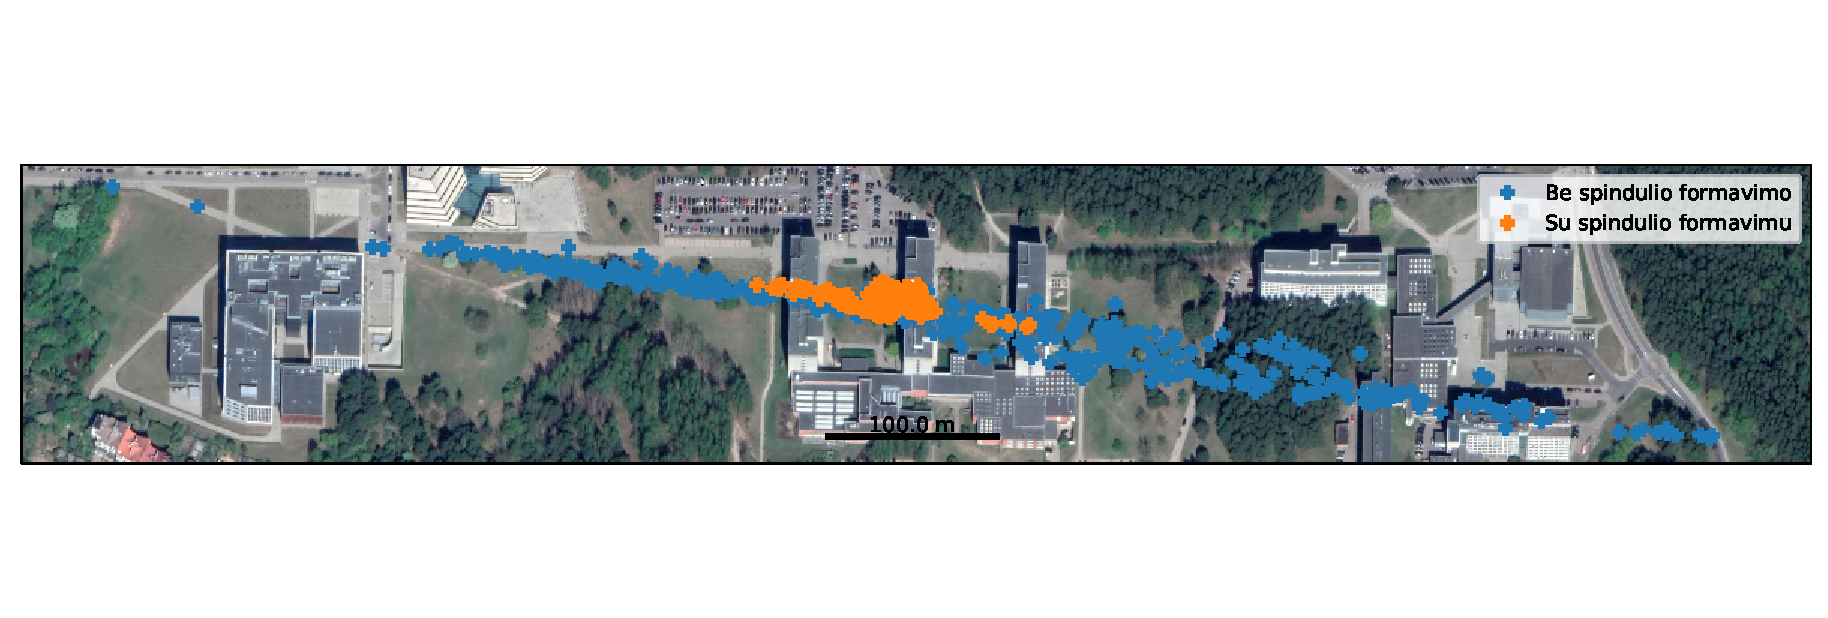
\includegraphics[scale=0.5]{drawings/two_reflections_map}
    \par\end{centering}
    \protect\caption{\label{fig:two_reflection_map}Imtuvo pozicijos koordinatės su spindulio formavimu ir be spindulio formavimo. Palydovinės nuotraukos \cite{google_maps}.}
\end{figure}

\subsubsection{GNSS imtuvo matavimų apibendrinimas}

% {sec:gnss_meas_no_reflection}
% {sec:gnss_meas_one_reflection}
% {sec:gnss_meas_two_reflection}

Atlikus tris matavimus, trijose skirtingose vietovėse, pademonstruota signalų
sklidimo kryp\-ties, bei atspindžių nustatymas pasinaudojant MUSIC algoritmu.
Pritaikius spindulio formavimą, pademonstruotas signalo triukšmo santykio padidėjimas nuo
$2\ \mathrm{dB}$ iki $8\ \mathrm{dB}$. Taikant spindulio formavimą
vietovėje, kurioje nėra atspindžių, nestebėtas koordinačių pasiskirstymo
sumažėjimas. Esant vienam atspindžių paviršiui, pastebėtas koordinatės 
nuokrypio sumažėjimas, bei vidutinės koordinatės atitolėjimas nuo atspindžių
šaltinio. Urbanistinėje aplinkoje spindulio formavimas padeda priimti
signalą iš didesnio skaičiaus palydovų kas leidžia patikslinti
koordinatės skai\-čia\-vi\-mą.

\end{document}
